\documentclass{handout}
\usepackage{handoutSetup}\usepackage{handoutShortcuts}

% Lines containing Private are excised when the public version of the document is created 

% Items within a Private environment are excised when the public version of the document is created

%\usepackage{endfloat}  % uncomment to put figures at the end

\begin{document}
\handoutHeader
\providecommand{\dmEqZero}{\ensuremath{\Delta\mRatE=0}}
\providecommand{\dcEqZero}{\ensuremath{\Delta\cRatE=0}}

\begin{verbatimwrite}{\jobname.title}
A Tractable Model of Buffer Stock Saving
\end{verbatimwrite}

\handoutNameMake

%\section{Introduction} 

This handout illustrates the logic of precautionary saving by assuming
that individuals face only a single, simple kind of uncertainty: A small risk of becoming permanently unemployed.  More realistic assumptions yield similar conclusions (after much more work).\footnote{The model simplifies many of the key results in \cite{carroll:brookings} and \cite{carrollBSLCPIH} using a  discrete-time version of the elegant continuous-time model of \cite{toche:urisk}.
  For a brief summary of the precautionary saving literature, see
  \cite{CarrollKimballPSPW}; for a more rigorous   treatment of the theoretical issues, see \cite{BufferStockTheory}.}

\section{The Microeconomic Consumer's Problem}
The aggregate wage $\Wage_{t}$ grows
by a constant factor $\WGro$ every period, reflecting exogenous labor productivity improvements:
\begin{equation}\begin{gathered}\begin{aligned}
        \Wage_{t+1} & =  \WGro \Wage_{t}.
\end{aligned}\end{gathered}\end{equation}

The consumer lives in a small open economy, with a constant interest factor $\Rfree$.  Defining $\mLevBF$ as
\textbf{m}arket resources (net worth plus current income), $\aLevBF$ as
end-of-period \textbf{a}ssets \textbf{a}fter \textbf{a}ll \textbf{a}ctions have been \textbf{a}ccomplished
(specifically, after the consumption decision), and $\bLevBF$ as \textbf{b}ank
\textbf{b}alances \textbf{b}efore receipt of labor income, the dynamic budget constraint (DBC) can be decomposed into the
following elements:
\begin{equation}\begin{gathered}\begin{aligned}
    \aLevBF_{t} & =  \mLevBF_{t}-\cLevBF_{t}
\\  \bLevBF_{t+1} & =  \Rfree \aLevBF_{t}
\\  \mLevBF_{t+1} & =  \bLevBF_{t+1}+\labor_{t+1}\Wage_{t+1}\empState_{t+1}  \label{eq:DBC}
\end{aligned}\end{gathered}\end{equation}
where $\labor$ measures the consumer's labor productivity
(`endowment') and $\empState$ is a dummy variable indicating the
consumer's employment state: Everyone is either
employed (state `e'), in which case $\empState = 1$, or unemployed
(state `u'), in which case $\empState=0$, so that for unemployed
individuals labor income is zero.\footnote{We could allow for
  unemployment insurance by modifying the values of $\empState$
  associated with the two states.  The key conclusions would not
  change.}

\pagebreak 
\subsection{The Unemployed Consumer's Problem} \label{subsec:Fred}

Once a person becomes unemployed, that person can never become
employed again (i.e.\ if $\empState_{t}=0$ then $\empState_{t+1}=0$).
Consumers have a CRRA felicity function\footnote{`Felicity' refers
  explicitly to a one-period, or in a continuous-time model, an
  instantaneous utility function.}
$\uFunc(\bullet)= \bullet^{1-\CRRA}/(1-\CRRA)$, and they discount
future felicity geometrically by $\Discount$ per period.


\renewcommand{\MPCU}{\MPC} % In principle, if parameters change when unemployed (like, death rate), could have different MPC; in practice, not done here
The solution to the unemployed consumer's optimization problem
is\footnote{See \handoutC{PerfForesightCRRA} for a derivation, noting that human wealth is zero for the unemployed consumer.} 
\begin{equation}\begin{gathered}\begin{aligned}
        \cLevBF^{u}_{t} & =  \underbrace{\left(1-\overbrace{\Rfree ^{-1}(\Rfree{\Discount})^{1/\CRRA}}^{\equiv \PatR}\right)}_{\equiv \MPCU} \bLevBF_{t} \label{eq:cpfinfhorunemp} %\label{eq:cdel} \label{eq:kappaDef} \label{eq:PatR}
,
\end{aligned}\end{gathered}\end{equation}
where the $u$ superscript signifies the consumer's (un)employment
status; $\MPCU$ is the marginal propensity to consume for the perfect
foresight consumer, which is strictly below the MPC for the problem
with uncertainty (\cite{carroll&kimball:concavity}); and $\PatR$ is
what \cite{BufferStockTheory} calls the `return patience factor.'\footnote{The Old English letter $\Pat = (\Rfree \Discount)^{1/\CRRA}$, which conveniently looks something like a combination of $\Rfree, \Discount, $ and $\CRRA$, is used to designate the `absolute patience factor' which determines whether consumption will rise ($\Pat > 1$), stay the same ($\Pat = 1$), or fall ($\Pat < 1$) in the perfect foresight problem (\handoutC{PerfForesightCRRA}).  Terms like this are all defined in \cite{carrollBSTheory} and citations to that paper will henceforth be omitted when new terms are introduced, on the understanding that the reader knows to see \cite{carrollBSTheory} for further definition and discussion.}


\indent We now impose the `return impatience condition' (RIC),
\begin{equation}\begin{gathered}\begin{aligned}
  \underbrace{\left(\frac{(\Rfree \Discount)^{1/\CRRA}}{\Rfree}\right)}_{= \PatR} < 1 \label{eq:RIC}
\end{aligned}\end{gathered}\end{equation}
which deserves its name because it is the condition that guarantees that $\MPCU
> 0$ -- the consumer must not be {\it so} patient that, given the interest rate, a boost to
resources fails to boost spending.\footnote{`Pathologically patient' consumers who do not satisfy this condition can be thought of as people who would hoard any incremental resources in order to enable even more extra spending in the distant future.}
An alternative (equally correct)
interpretation is that the condition guarantees that the PDV of
consumption for the unemployed consumer is not infinity.\footnote{For a perfect
foresight consumer, \handoutC{PerfForesightCRRA} shows that consumption grows by the factor
$\Pat = (\Rfree\Discount)^{1/\CRRA}$, so if we do not impose the RIC, consumption would `want' to grow by
a factor greater than the factor $\Rfree$ by which it is being
discounted.}  

For many purposes (not least, the calibration of the model), it turns out to be useful to alternatviely express
impatience conditions like \eqref{eq:RIC} in terms of the upper bound of the range of time preference
factors $\bar{\Discount}$ that satisfy the condition; solving \eqref{eq:RIC} for $\Discount$, we designate this 
object \providecommand{\DiscountMaxRIC}{\ensuremath{\bar{\Discount}_{\text{RIC}}}}
\begin{equation}\begin{gathered}\begin{aligned}
  \DiscountMaxRIC & =  \Rfree^{\CRRA-1}
\end{aligned}\end{gathered}\end{equation}
and write the alternative version of the constraint as 
\begin{equation}\begin{gathered}\begin{aligned}
  \Discount & <  \DiscountMaxRIC \label{eq:DiscountMaxRIC}.
\end{aligned}\end{gathered}\end{equation}

$\PatR$ is the `return patience factor' because it defines the patience factor $\Pat$
relative to the return factor $\Rfree$; correspondingly, we define the `return
patience rate' as lower-case
\begin{equation}\begin{gathered}\begin{aligned}
   \patr & \equiv   \log \PatR \label{eq:patr}
\\ & \approx \PatR - 1 
\\ & =  -\MPCU
\end{aligned}\end{gathered}\end{equation}
and we say that a consumer is `return impatient' if the RIC \eqref{eq:RIC} holds (equivalent conditions are $\patr < 0$ and $\MPCU > 0$).\footnote{Throughout, we will casually treat logs of factors like $\PatR$ as equivalent to the level minus 1; that is, we will treat expressions like those in \eqref{eq:patr} as interchangeable, which is an appropriate approximation so long as the factor is `close' to 1.}

\subsection{The Employed Consumer's Problem}

\subsubsection{Unemployment Risk as a Mean Preserving Spread in Human Wealth} \label{subsubsec:uMPS}
If a person who is employed in period $t$ ($\empState_{t}=1$) is still employed next
period ($\empState_{t+1}=1$), market resources will be
\begin{equation}
\mLevBF^{e}_{t+1} = (\mLevBF^{e}_{t}-\cLevBF^{e}_{t})\Rfree+\Wage_{t+1}\labor_{t+1}. \label{eq:Metp1}
\end{equation}

But employed consumers face a constant risk $\urate$ of becoming unemployed.  
It will be convenient to define $\erate\equiv 1-\urate$ as the probability that a consumer does {\it not} become unemployed.  Whether the consumer is employed or not, his labor productivity $\labor$ is well-defined:\footnote{`Labor productivity' is purely hypothetical for a consumer who is unemployed; but defining it even for unemployed consumers simplifies notation and some later analysis.}  For convenience, $\labor$ is assumed to grow by a factor $\erate^{-1}$ every period,
\begin{equation}
\labor_{t+1} =    \labor_{t}/\erate \label{eq:meanPreserve},
\end{equation}
which means that for a consumer who remains employed, labor income will grow by factor
\begin{equation}\begin{gathered}\begin{aligned}
  \PGro & =  \WGro/\erate
\end{aligned}\end{gathered}\end{equation}
so that the {\it expected} labor income growth factor for
employed consumers is the same $\WGro$ as in the perfect foresight case:
\begin{equation*}\begin{gathered}\begin{aligned}
  \Ex_{t}[\Wage_{t+1}\labor_{t+1}\empState_{t+1}] & =   \left(\frac{\labor_{t} \WGro \Wage_{t}}{\erate}\right)\left(\urate \times 0 + \erate \times 1 \right)
\\ \left(\frac{\Ex_{t}[\Wage_{t+1}\labor_{t+1}\empState_{t+1}]}{\Wage_{t} \labor_{t}}\right) &  =  \WGro
,
\end{aligned}\end{gathered}\end{equation*}
which is  the reason for \eqref{eq:meanPreserve}'s assumption about the growth of
individual labor productivity: It implies
that an increase in $\urate$ is a pure increase in uncertainty with no
effect on the PDV of expected labor income (`human wealth'); an increase in $\urate$ therefore constitutes a `mean-preserving spread' in human wealth.

\subsubsection{First Order Optimality Condition}

The same solution methods used in \handoutC{PerfForesightCRRA} can 
be applied here too (take the first order condition with respect to $\cLev$, use
the \handoutC{Envelope} theorem); the only difference is the need to keep the expectations operator
in place.  Using $\bullet$ as a placeholder for `e' or `u,' the
usual steps lead to the standard consumption Euler equation:
\begin{equation}\begin{gathered}\begin{aligned}
        \uFunc^{\prime}(\cLevBF^{e}_{t}) & =  \Rfree\Discount \Ex_{t}\left[\uFunc^{\prime}(\cLevBF^{\bullet}_{t+1}) \right]
\\  1         & =  \Rfree\Discount \Ex_{t}\left[\left(\frac{\cLevBF^{\bullet}_{t+1}}{\cLevBF^{e}_{t}}\right)^{-\CRRA} \right]
%\\  & =  \Rfree\Discount \left[\urate \left(\frac{\cLevU_{t+1}}{\cLevBF^{e}_{t}}\right)^{-\CRRA}+\erate\left(\frac{\cLevBF^{e}_{t+1}}{\cLevBF^{e}_{t}}\right)^{-\CRRA} \right]
.
\end{aligned}\end{gathered}\end{equation}

Defining nonbold variables as the bold equivalent divided
by the level of permanent labor income for an employed consumer, e.g.\ ${\cRat}^{e}_{t}=\cLevBF^{e}_{t}/(\Wage_{t}\labor_{t})$, we can rewrite the
consumption Euler equation as
\begin{equation}\begin{gathered}\begin{aligned}
  1         & =  \Rfree\Discount \Ex_{t}\left[\left(\frac{{c}^{\bullet}_{t+1} \Wage_{t+1}\labor_{t+1}}{{\cRat}^{e}_{t} \Wage_{t}\labor_{t}}\right)^{-\CRRA} \right]  
\\          & =  \Rfree\Discount \Ex_{t}\left[\left(\frac{{c}^{\bullet}_{t+1}}{{\cRat}^{e}_{t}}\PGro\right)^{-\CRRA} \right]
\\          & =  \PGro^{-\CRRA}\Rfree\Discount \Ex_{t}\left[\left(\frac{{c}^{\bullet}_{t+1}}{{\cRat}^{e}_{t}}\right)^{-\CRRA} \right] 
\\          & =  \PGro^{-\CRRA}\Rfree\Discount \left\{(1-\urate)\left(\frac{{\cRat}^{e}_{t+1}}{{\cRat}^{e}_{t}}\right)^{-\CRRA}+\urate \left(\frac{\cU_{t+1}}{{\cRat}^{e}_{t}}\right)^{-\CRRA}\right\} \label{eq:Explicit}.
\end{aligned}\end{gathered}\end{equation}


\subsubsection{Analysis and Intuition of Consumption Growth}
It will be useful now to define a `growth patience factor' (this terminology will be justified below):
\begin{equation}\begin{gathered}\begin{aligned}
  \GPFacRaw & =  \left(\frac{(\Rfree\Discount)^{1/\CRRA}}{\PGro}\right), \label{eq:GPFacRaw}
\end{aligned}\end{gathered}\end{equation}
which is the factor by which ${\cRat}^{e}$ would grow in the
perfect foresight version of the model with permanent income growth factor
$\PGro$ (again see \handoutC{PerfForesightCRRA}).  
Using this,
\eqref{eq:Explicit} can be written as\footnote{This is where the perfect foresight assumption is important; without it \eqref{eq:BeforePFStep} would be 
\begin{equation}\begin{gathered}\begin{aligned}
 1       & =  \GPFacRaw^{\CRRA} \Ex_{t}\left[\left(\frac{{\cRat}^{e}_{t+1}}{{\cRat}^{e}_{t}}\right)^{-\CRRA} \left\{1+\urate\left[\left(\frac{\cU_{t+1}}{{\cRat}^{e}_{t+1}}\right)^{-\CRRA}-1\right]\right\}\right] \label{eq:BeforePFStepWithEx}
\end{aligned}\end{gathered}\end{equation}
and we would be unable to proceed to the step from \eqref{eq:BeforePFStep} to \eqref{eq:ctp1Oct}.}

\begin{equation}\begin{gathered}\begin{aligned}
        1  & = \GPFacRaw^{\CRRA} \left(\frac{{\cRat}^{e}_{t+1}}{{\cRat}^{e}_{t}}\right)^{-\CRRA} \left\{(1-\urate)+\urate\left[\left(\frac{\cU_{t+1}}{{\cRat}^{e}_{t}}\right)\left(\frac{{\cRat}^{e}_{t}}{{\cRat}^{e}_{t+1}}\right)\right]^{-\CRRA}\right\}
\\       & = \GPFacRaw^{\CRRA} \left(\frac{{\cRat}^{e}_{t+1}}{{\cRat}^{e}_{t}}\right)^{-\CRRA} \left\{1+\urate\left[\left(\frac{\cU_{t+1}}{{\cRat}^{e}_{t+1}}\right)^{-\CRRA}-1\right]\right\} \label{eq:BeforePFStep}
\\       \left(\frac{{\cRat}^{e}_{t+1}}{{\cRat}^{e}_{t}}\right)^{\CRRA} & = \GPFacRaw^{\CRRA} \left\{1+\urate\left[\left(\frac{{\cRat}^{e}_{t+1}}{\cU_{t+1}}\right)^{\CRRA}-1\right]\right\} \label{eq:ctp1Oct}
\\       \left(\frac{{\cRat}^{e}_{t+1}}{{\cRat}^{e}_{t}}\right) & = {\GPFacRaw} \left\{1+\urate\left[\left(\frac{{\cRat}^{e}_{t+1}}{\cU_{t+1}}\right)^{\CRRA}-1\right]\right\}^{1/\CRRA}. \label{eq:cedel}
\end{aligned}\end{gathered}\end{equation}

\opt{MarginNotes}{\marginpar{\tiny Mnemonics for $\nabla$: sort of like a change, but a downward change, so like $\Delta$, but points down.}}

\opt{MarginNotes}{\marginpar{\tiny Obviously ${\cRat}^{e}_{t+1} > \cU_{t+1}$ so $\nabla {\cRat}^{e}_{t+1} > 0$.}}

Now define $\nabla _{t+1} \equiv
\left(\frac{{\cRat}^{e}_{t+1}-\cU_{t+1}}{\cU_{t+1}}\right)$ (which is
the proportion by which consumption would
be greater next period for an employed than for an 
unemployed person), and define an `excess prudence' factor
\begin{equation}\begin{gathered}\begin{aligned}
  \prudEx & =  \left(\frac{\CRRA-1}{2}\right).
\end{aligned}\end{gathered}\end{equation}

Appendix~\ref{sec:CGroApprox} shows that, with some approximations, we can rewrite \eqref{eq:cedel} as
\begin{equation}\begin{gathered}\begin{aligned}
         \left(\frac{{\cRat}^{e}_{t+1}}{{\cRat}^{e}_{t}}\right) & \approx  \left(1+ \urate (1+\prudEx\nabla _{t+1})\nabla _{t+1}\right) {\GPFacRaw}
         \label{eq:cedelapprox}
\end{aligned}\end{gathered}\end{equation}
which can be simplified in the logarithmic utility case (where $\prudEx = 0$) to
\begin{equation}\begin{gathered}\begin{aligned}
         \left(\frac{{\cRat}^{e}_{t+1}}{{\cRat}^{e}_{t}}\right) & \approx  \left(1+ \urate \nabla _{t+1}\right) {\GPFacRaw} \label{eq:cedelapproxLog}. 
\end{aligned}\end{gathered}\end{equation}

Now since consumption if employed ${\cRat}^{e}_{t+1}$ is surely greater than
consumption if unemployed $\cU_{t+1}$, $\nabla _{t+1}$ is
certainly a positive number.  But since ${\GPFacRaw}$ is the
value that ${\cRat}^{e}_{t+1}/{\cRat}^{e}_{t}$ would exhibit in a perfect
foresight model, this equation tells us that uncertainty boosts
consumption growth\footnote{At least, for continuing-employed consumers.} -- in the logarithmic
case, consumption growth is augmented by an amount
proportional to the probability of becoming unemployed $\urate$ multiplied
by the size of the `consumption risk' (the amount by which consumption
would fall if unemployment occurs).


As noted above, for any given $\mRatE_{t}$, an increase in uncertainty
constitutes a mean-preserving spread in human wealth; thus the `human
wealth effect' of an increase in $\urate$ would be zero for a consumer
without a precautionary motive.  In this small-open-economy model a
change in $\urate$ also has no effect on the interest rate $\rfree$,
and so none of the conventional determinants of consumption in the
perfect foresight model (the income, substitution, and human wealth
effects) is affected by a change in uncertainty.  The increase in consumption
growth from an increase in $\urate$ in
\eqref{eq:cedelapprox} or \eqref{eq:cedelapproxLog} therefore must be
entirely the result of the precautionary motive.  Furthermore, because 
a profile with faster consumption {\it growth} can only exhibit the {\it same PDV} if that faster growth 
{\it starts} from a lower initial consumption {\it level}, we know that for any given initial value of $\mRatE$, the introduction of a risk
of becoming unemployed $\urate$ induces a (precautionary) decline in consumption (and corresponding increase in
saving).

Furthermore, under the (compelling) assumption that $\CRRA > 1$, \eqref{eq:cedelapprox} implies that a consumer with
a higher degree of prudence (larger $\CRRA$ and therefore larger $\prudEx$) will
anticipate a greater increment to consumption growth as a consequence of the introduction of uncertainty.  This reflects the greater precautionary
saving motive induced by a higher degree of prudence.

\opt{MarginNotes}{\marginpar{\tiny They should have seen phase diagrams in Maccini's course.  Remind them what it is.}}


\subsubsection{Finding the Target}

The target level of $\mRat^{e}$ (if one exists) will be the point of intersection between the $\dcEqZero$ and $\dmEqZero$ loci.  \opt{MarginNotes}{\marginpar{\tiny Note the dropping of the $t+1$ subscripts because we're talking about a steady-state.}}

The $\dcEqZero$ locus can be characterized by substituting ${\cRat}^{e}_{t+1}={\cRat}^{e}_{t} \equiv {\cRat}^{e}$ into \eqref{eq:cedel}:
\begin{equation}\begin{gathered}\begin{aligned}
         1 & = \left\{1+\urate\left[\left(\frac{{\cRat}^{e}_{t+1}}{\cRat_{t+1}^{u}}\right)^{\CRRA}-1\right]\right\} \GPFacRaw^{\CRRA} \label{eq:ctp1OctEq1}
\\ \GPFacRaw^{-\CRRA} & =  (1-\urate)+\urate\left(\frac{{\cRat}^{e}_{\tSS}}{\cRat_{t+1}^{u} }\right)^{\CRRA}
\\ \underbrace{\left(\frac{\GPFacRaw^{-\CRRA}-1+\urate}{\urate}\right)^{1/\CRRA}}_{\equiv \straight} & =   \left(\frac{{\cRat}^{e}_{\tSS}}{\cRatU_{t+1}}\right) \label{eq:straightDef}
\\ \underbrace{\left(\overbrace{\urate^{-1}(\GPFacRaw^{-\CRRA}-1)}^{\equiv \varpi}+1\right)^{1/\CRRA}}_{\straight=(1+\varpi)^{1/\CRRA}} & =   \left(\frac{{\cRat}^{e}_{\tSS}}{\cRatU_{t+1}}\right) \label{eq:varpiDef}
\\      {\cRat}^{e}_{\tSS} & = \cRat^{u}_{t+1} \straight \label{eq:cRatEtfmcRatUtp1}.
\end{aligned}\end{gathered}\end{equation}


The importance of the linearity of the consumption function of the unemployed consumer now becomes evident:  It means that the RHS of \eqref{eq:cRatEtfmcRatUtp1} is linear in $\cRat^{e}_{t}$:
\begin{equation}\begin{gathered}\begin{aligned}
  \cRat^{e}_{t} & =  \overbrace{(\mRat^{e}_{t}-{\cRat}^{e}_{t})\Rnorm \MPCU}^{\cRat^{u}_{t+1}} \straight \label{eq:PSTerm}.
\end{aligned}\end{gathered}\end{equation}


We know that $\mRatE_{t}-{\cRat}^{e}_{t} > 0$ because a consumer in these
circumstances (facing possible perpetual unemployment) will never
borrow (see below for a full discussion of this point). 
Since the RIC imposes $\MPCU>0$, \eqref{eq:PSTerm} tells
us that steady-state consumption (if it exists)\footnote{Under some parameter values, the model has solutions under which the consumer always spends less than the amount that would leave $\mRatE$ constant, and so accumulates forever.} is a positive finite number so long as $(1+\varpi)^{1/\CRRA}=\straight > 0$, which will hold true iff the numerator on the LHS of
\eqref{eq:straightDef} is a positive finite number; that is, we need the
condition:
\begin{equation}\begin{gathered}\begin{aligned}
        \PGro^{\CRRA}(\Rfree\Discount)^{-1}-(1-\urate) & >  0  \\
       \PGro^{\CRRA} & >  (\Rfree \Discount (1-\urate))
\\     1 & >  \left(\frac{(\Rfree \Discount (1-\urate))^{1/\CRRA}}{\PGro}\right) = \GPFacRaw (1-\urate)^{1/\CRRA} 
  \label{eq:GICExistsSoln} %\label{eq:GICTBS}
.\end{aligned}\end{gathered}\end{equation}

\hypertarget{GIFMax}{}\hypertarget{DiscountMaxGICTBS}{}

\subsubsection{Upper Bounds for $\Discount$, Given Other Parameters}


As with the RIC, it may be useful to rewrite this as defining an upper bound to the permissible time preference rates: \providecommand{\DiscountMaxGICTBS}{\bar{\Discount}_{\text{TBS}}}
\begin{equation}\begin{gathered}\begin{aligned}
\Discount < \DiscountMaxGICTBS & =  \left(\frac{\PGro^{\CRRA}}{\Rfree(1-\urate)}\right) \label{eq:DiscountMaxGICTBS}
.
\end{aligned}\end{gathered}\end{equation}

\providecommand{\GICPGro}{GIC$_{\PGro}$}
\providecommand{\GICWGro}{GIC$_{\WGro}$}
In the limit as $\urate$ approaches zero, \eqref{eq:GICExistsSoln} reduces to a requirement that the growth patience factor is less than one,
\begin{equation}\begin{gathered}\begin{aligned}
  \GPFacRaw & <  1 \label{eq:GICPGro}
,\end{aligned}\end{gathered}\end{equation}
which, as in \handoutM{PerfForesightCRRA},  we call a `growth impatience condition' (GIC) by analogy to the `return impatience condition' \eqref{eq:RIC} imposed earlier.  \handoutC{PerfForesightCRRA} shows that the limit of \eqref{eq:GICExistsSoln} as $\urate \downarrow 0$, $\WGro > \Pat$, ensures that a consumer facing no uncertainty is sufficiently impatient that his wealth-to-permanent-income ratio will fall over time.  
We label the weaker condition \eqref{eq:GICExistsSoln} the `GIC-TBS' (the version of the GIC required for a solution to exist in the Tractable Buffer Stock model).  It will always hold if the plain-vanilla \GICWGro~holds because $\urate \geq 0$.  Thus, a consumer who, in the absence of uncertainty, would satisfy both the RIC and the \GICWGro, will have a positive finite target level of wealth when uncertainty is introduced.  (See appendix~\ref{sec:mTargExists} for a proof that the \GICPGro~condition is both necessary and sufficient for the existence of a target level of wealth.)

When it is useful to distinguish the version of the GIC that applies in the model with income growth of $\WGro$ from the corresponding condition when growth is $\PGro$ we will label the two conditions \GICPGro~and \GICWGro, and the corresponding bounds on $\Discount$ are 
\providecommand{\DiscountMaxGICPGro}{\bar{\Discount}_{\text{GIC}_\PGro}}
\providecommand{\DiscountMaxGICWGro}{\bar{\Discount}_{\text{GIC}_\WGro}}
\begin{equation}\begin{gathered}\begin{aligned}
   \Discount < \DiscountMaxGICPGro & =  \Rfree^{\CRRA-1}\PGro^{\CRRA}
\\ \Discount < \DiscountMaxGICWGro & =  \Rfree^{\CRRA-1}\WGro^{\CRRA}
\end{aligned}\end{gathered}\end{equation}



Using $\pGro \equiv \log \PGro$, we similarly define the corresponding `growth impatience rate':
\begin{equation}\begin{gathered}\begin{aligned}
  \patpGro & \equiv  \log \GPFacRaw \approx \CRRA^{-1}(\rfree-\timeRate) - \pGro
\end{aligned}\end{gathered}\end{equation}
so that the growth impatience condition \eqref{eq:GICExistsSoln} (the GIC-TBS) can also be written (approximately) as
\begin{equation}\begin{gathered}\begin{aligned}
  \patpGro - \CRRA^{-1}\urate & <  0   \label{eq:GICrateUsingpGro}
\end{aligned}\end{gathered}\end{equation}
or, since $\pGro \approx \wGro+\urate$, 
\begin{equation}\begin{gathered}\begin{aligned}
 \CRRA^{-1}(\rfree-\timeRate-\urate)-(\wGro+\urate) & <  0 \label{eq:GICrateUsingwGro}
.
\end{aligned}\end{gathered}\end{equation}

\subsubsection{Why Increased Unemployment Risk Increases Effective Growth Impatience}

Equation \eqref{eq:GICrateUsingwGro} becomes easier to satisfy as $\urate$ increases, since 
in both places where $\urate$ appears on the LHS it is with a negative coefficient.

The reason the two appearances of $\urate$ have not been combined in \eqref{eq:GICrateUsingwGro} is that the separate 
terms reflect two logically distinct effects.  The first appearance, where $\urate$ is premultiplied by $-\CRRA^{-1}$, 
can be interpreted as capturing the sense in which an increase in $\urate$ is like an increase in the discounting of the future (the
coefficient on $\urate$ is the same as that on $\timeRate$).  This downweighting of the future occurs precisely because that future
might not occur (if the consumer becomes unemployed).\footnote{A different future -- with the consumer unemployed -- does occur; but here we are effectively analyzing the behavior of a consumer {\it contingent on that consumer remaining employed}.}  The effect is much like the increase in discounting that occurs 
when a positive probability of death is introduced in consumption problems, cf.~\cite{blanchardFinite}.

The second, separate, reason $\urate$ weakens growth impatience (that is, the GIC-TBS holds in more circumstances than the \GICWGro) is that we adjust labor productivity growth so that $\pGro=\wGro+\urate$ in 
order to maintain constant human wealth for different values of
$\urate$ (eq.\ \eqref{eq:meanPreserve}).  For higher
$\urate$, permanent income growth is greater {\it conditional on
  remaining employed}; the continuously-employed consumer is effectively
more `impatient' in the relevant sense of desiring consumption growth
slower than income growth.

This is essentially a mechanical result, which reflects our model's
design for the purpose of examining thought experiments that
manipulate the degree of uncertainty while leaving the
perfect-foresight level of human wealth constant.  

Note that although $\urate$ is our measure of uncertainty, neither of 
these effects of $\urate$ is in any meaningful sense directly a 
`precautionary' effect; instead, they both reflect effects of 
$\urate$ on the relevant degree of growth impatience in the GIC-TBS 
condition.  

\subsubsection{The Target Level of $\mRatE$}
\renewcommand{\tSS}{\null}

Appendix~\ref{sec:mTargExists} demonstrates that the RIC and the GIC-TBS are necessary conditions for the existence of a target value of market resources $\mTarg^{e},$ and that the \GICPGro~is sufficient.   Appendix~\ref{sec:mTargExact} solves for an explicit formula for that target.

Briefly, this is accomplished as follows.  We can obtain the $\dcEqZero$ locus by substituting
${\cRat}^{e}_{\tNow+1}={\cRat}^{e}_{\tNow}={\cRat}^{e}$ into equation \eqref{eq:PSTerm}:
\begin{equation}\begin{gathered}\begin{aligned}
  {\cRat}^{e}_{\tSS} & =  \mRatE_{\tSS} \Rnorm\MPCU\straight - {\cRat}^{e}_{\tSS} \Rnorm\MPCU\straight
\\  {\cRat}^{e}_{\tSS} & =  \left(\frac{\Rnorm\MPCU\straight}{1+\Rnorm\MPCU\straight}\right)\mRatE
  \label{eq:cDelEqZero} %\label{eq:DceEq0}
\end{aligned}\end{gathered}\end{equation}

Now we need to use a normalized version of the DBC (equation \eqref{eq:Metp1}),
\begin{equation}\begin{gathered}\begin{aligned}
        \mRatE_{t+1} & =  (\mRatE_{t}-{\cRat}^{e}_{t})\Rnorm+1 \label{eq:metp1}
\end{aligned}\end{gathered}\end{equation}
to derive the $\mRatE_{t+1}=\mRatE_{t}=\mRatE_{\tSS}$ locus (also referred
to as the $\dmEqZero$ locus): \opt{MarginNotes}{\marginpar{\tiny Lack of time subscript indicates constancy.}}
\begin{equation}\begin{gathered}\begin{aligned}
%        \mRatE & =  (\mRatE-{\cRat}^{e})\Rnorm+1
      \Rnorm^{-1}(\mRatE_{\tSS}-1) & =  \mRatE_{\tSS}-{\cRat}^{e}_{\tSS}
\\      {\cRat}^{e}_{\tSS} & =  \mRatE_{\tSS}-\Rnorm^{-1}(\mRatE_{\tSS}-1)
\\       & =  (1-\Rnorm^{-1})\mRatE_{\tSS}+\Rnorm^{-1}. \label{eq:mDelEqZero}
\end{aligned}\end{gathered}\end{equation}

The steady-state levels of $\mRatE$ and ${\cRat}^{e}$ are the values of these two variables at which both
\eqref{eq:mDelEqZero} and \eqref{eq:cDelEqZero} hold.  This is
just a set of two linear equations and two unknowns, and with a bit of 
algebra can be solved explicitly.

In the special case of logarithmic utility ($\CRRA = 1$), the
appendix shows that (under some strong assumptions) an approximation to target market resources will be given by
\begin{equation}\begin{gathered}\begin{aligned}
 \mTarg^{e} & \approx  1 + \left(\frac{1}{(\pGro-\rfree)+\timeRate(1+(\pGro+\timeRate-\rfree)/\urate)}\right) \label{eq:mTargetLogCase}
\end{aligned}\end{gathered}\end{equation}
and that the GIC and the RIC guarantee that the denominator of the fraction is a positive number.

This expression encapsulates several of the key intuitions of the model.  The
`human wealth effect' of growth (cf.\ \cite{summersCapTax}) is captured by the first $\pGro$ term in the denominator;
clearly, for any calibration for which the denominator is a positive number, increasing
$\pGro$ will increase the size of the denominator and therefore reduce the target
level of wealth.  The human wealth effect of interest rates is  correspondingly captured
by the $-\rfree$ term.  An increase in the future discounting rate, $\timeRate$, will also
increase the size of the denominator and therefore reduce target wealth.  Finally,
a reduction in unemployment risk will boost $(\pGro+\timeRate-\rfree)/\urate$ and therefore reduce target
wealth.\footnote{$(\pGro+\timeRate-\rfree) > 0$ is guaranteed by \eqref{eq:GICrateUsingwGro} under $\log$ utility ($\CRRA=1$).}

The assumption of log utility is restrictive, and probably does not capture
sufficient aversion to consumption fluctuations.  Fortunately, another special
case helps to illuminate the effect of higher levels of prudence.  The appendix shows that, in the special case where $\timeRate=\rfree$, the
target level of wealth will be approximable by
\begin{equation}\begin{gathered}\begin{aligned}
 \mTarg^{\null} & \approx  1 + \left(\frac{1}{(\pGro-\rfree)+\timeRate(1+(\pGro/\urate)(1-(\pGro/\urate)\prudEx))}\right) \label{eq:mTargetrEqdelta}
\end{aligned}\end{gathered}\end{equation}
which is like \eqref{eq:mTargetLogCase} (with $\timeRate-\rfree=0$) but with the addition of the final term involving $\prudEx$ which measures the amount by which prudence exceeds the logarithmic benchmark.
An increase in $\prudEx$ reduces the denominator of \eqref{eq:mTargetrEqdelta}
and thereby boosts the target level of wealth: Exactly what would be expected from
an increase in the intensity of the precautionary motive.

Note that the different effects {\it interact} with each other, in the
sense that the strength of, say, the human wealth effect will vary
depending on the values of the other parameters.  The ways in which
these interactions make intuitive sense will repay deep reflection.
(Hint: How much I care about the future governs the power that future
events have in determining my targets; use the formula to think about why).

\subsubsection{Conditions Required for a Perfect Foresight Solution; Existence of Target Value of $\mRatE$}

Interestingly, the limit of the buffer stock model as $\urate \downarrow 0$ is {\it not} the perfect foresight solution obtained when $\urate$ is exactly equal to zero.  But that limiting solution contains most of the insight that comes from the more general model with $\urate$ bounded strictly away from zero, so we confine the analysis here to that limiting case. 

\providecommand{\FHWCPGro}{FHWC$_{\PGro}$}
\providecommand{\FHWCWGro}{FHWC$_{\WGro}$}
The handout \handoutC{PerfForesightCRRA} shows that in the perfect foresight context, it is necessary to impose the Finite Human Wealth Condition $\Rfree > \WGro$ (henceforth, \FHWCWGro) to obtain a sensible solution.\footnote{The appendix to \handoutC{PerfForesightCRRA} shows that if the \FHWCWGro~fails, the limit of the perfect foresight model is $\cFunc(\mRat)=\infty~\forall~\mRat$, which is not a useful or plausible solution.}  But if the \FHWCWGro~holds, the \GICWGro~is strictly stronger than the RIC, because the combination $\Pat/\WGro < 1$ and $\Rfree > \WGro$ obviously implies $\Pat/\Rfree < 1$.  If we substitute $\PGro$ for $\WGro$, we can define the corresponding version of the condition in the case where growth is $\PGro$: the \FHWCPGro.

It turns out that in the buffer stock model, we can relax the requirement that human wealth is finite.  

We pointed out above that \eqref{eq:GICExistsSoln}, which is necessary for the existence of a steady-state level of consumption, implies that the \GICPGro~holds in the case being considered here, the limit as $\urate \downarrow 0$.  The interesting question is therefore what happens when the \FHWCWGro~does not hold (that is $\WGro > \Rfree$).  

Given that the \GICWGro~holds, if the \FHWCWGro~does not hold the RIC may or may not hold:  $\WGro > \Rfree$ implies that $\Pat/\Rfree > \Pat/\WGro$ but $1 > \Pat/\WGro$ could be consistent with $\Pat/\Rfree$ being greater or less than one.  But recall that our assumption is that the unemployed consumer is assumed to behave according to the perfect foresight model with human wealth equal to zero.  We must therefore impose the RIC in order to obtain a nondegenerate solution.  We therefore impose the RIC.

For any finite horizon, human wealth is finite, and there is a positive probability that income will be zero over the remainder of the horizon.  This puts a strict bound on the extent to which consumers are willing to rely for current consumption upon future income that is unbounded in expectation (as the horizon extends) but potentially bounded in practice.  In effect, the precautionary motive introduces a self-imposed borrowing constraint that prevents the (arbitrarily large) amount of future income from being something the consumer is willing to borrow against.

The consequence is that the limiting model (as $\urate \downarrow 0$) exhibits a solution with a unique finite target $\mRatE$ so long as \eqref{eq:GICExistsSoln} holds, {\it even if human wealth is infinite}; in this case the $\dmEqZero$ locus is downward sloping (because $1-\Rnorm^{-1}<1$; see \eqref{eq:mDelEqZero}) while the $\dcEqZero$ locus is upward sloping (as guaranteed by \eqref{eq:GICExistsSoln}).  Thus, a target $\mRatE$ will exist.

\subsubsection{The Phase Diagram}

Figure~\ref{fig:PhaseDiag} presents the phase diagram.
\begin{figure}
\caption{Phase Diagram}\label{fig:PhaseDiag}
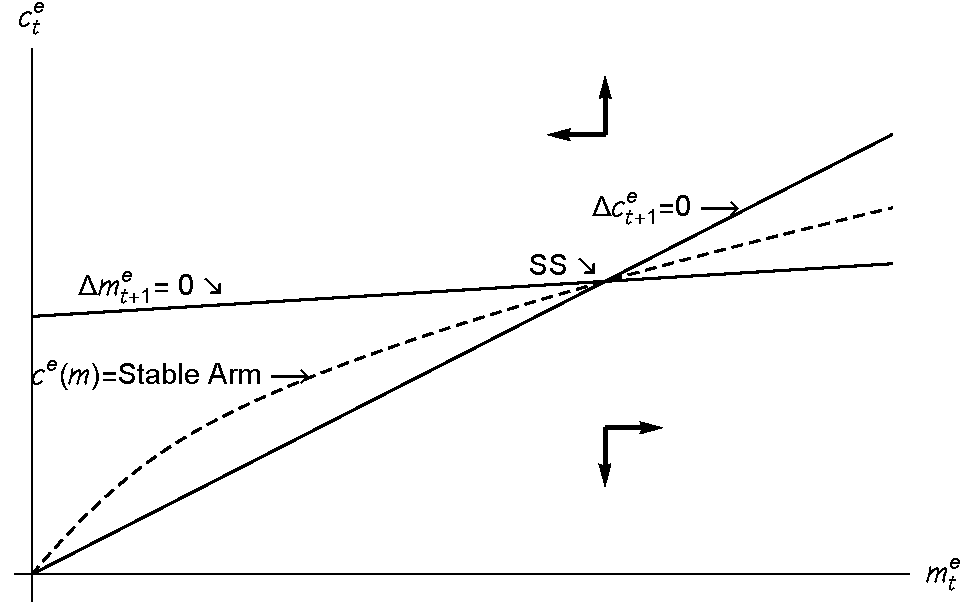
\includegraphics[width=6in]{../Figures/TractableBufferStockPhaseDiag}
\end{figure}


The $\Delta \mRatE_{\tSS} = 0$ locus, given in \eqref{eq:mDelEqZero},
indicates, for a given level of $\mRatE_{\tSS}$, how much consumption
${\cRat}^{e}_{\tSS}$ would be exactly the right amount to leave $\mRatE$
unchanged.  Call this the `permanently sustainable consumption locus,' or for short `sustainable consumption.'\footnote{Some authors refer to $\Delta \mRatE_{\tSS} = 0$ as giving the level of `permanent income,' but this definition differs from \cite{friedmanATheory}'s and is 
problematic because it could be confused with `permanent labor income' $\Wage_{t} \labor_{t}$.}  For any given $\mE$, consuming an amount less than the `sustainable' level will cause wealth will rise (and conversely for points above $\Delta \mRatE =0$).  This provides the logic for
the horizontal arrows of motion in the diagram: Above the sustainable consumption locus
they point left, and below they point right.

\opt{MarginNotes}{\marginpar{\tiny READ THIS PARAGRAPH CAREFULLY BEFORE LECTURE.  Recall that $\Delta {\cRat}^{e}$ condition is derived from Euler equation (preferences); can't use budget constraint logic here (that's in the $\Delta \mRatE$ locus).}}

The intuition for the $\Delta {\cRat}^{e}_{\tSS}=0$ locus (which comes from
\eqref{eq:cDelEqZero}) is a bit subtler.  Take a point on 
the $\Delta {\cRat}^{e}_{\tSS}=0$ locus, and consider how things 
would change if $\mE$ were a bit higher at the same $\cE$.  
Recall that the growth rate of consumption consistent with 
the Euler equation \eqref{eq:cedel} depends on the amount by which consumption will
fall if the bad state is realized, $\nabla_{t+1} = \cE_{t+1}/\cU_{t+1}$.  
But $\cU_{t+1} = \MPCU \Rfree (\mE_{t} - \cE_{t})$ so at the same $\cE_{t}$ but 
a greater $\mE_{t}$, $\cU_{t+1}$ will be larger.  If $\cE_{t+1}$ were to remain
unchanged, then with the larger $\cU_{t+1}$ the ratio $\nabla_{t+1} = \cE_{t+1}/\cU_{t+1}-1$ would be smaller.

The consequences of this are easiest to see in the logarithmic case whose consumption growth equation is derived in \eqref{eq:cedelapproxLog}, which tells us that ${\cRat}^{e}_{t+1} \approx {\cRat}^{e}_{t}\left(1+ \urate \nabla _{t+1}\right) {\GPFacRaw}$, which directly 
implies that the lower $\nabla_{t+1}$ will yield a lower $\cE_{t+1}$.  That is, for any point to the right of the $\Delta \cE_{t+1}=0$ locus, the growth rate of consumption will be lower than at the corresonding point on the locus.  Since on the locus, growth
was zero, this means that to the right of the locus, $\cE$ is declining (hence the down arrow in the phase diagram).  Reciprocally, for any point to the left of $\Delta \cE_{t+1}=0$, the Euler equation implies that consumption will rise.


\begin{figure}
\caption{The Consumption Function}\label{fig:cFunc}
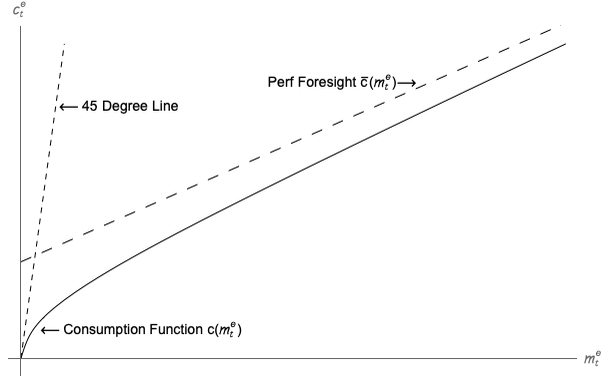
\includegraphics[width=6in]{../Figures/TractableBufferStockcFunc}
\end{figure}

\subsubsection{The Consumption Function}
The next figure shows the optimal consumption function $\cFunc(m)$ for an
employed consumer (dropping the $e$ superscript to reduce clutter).  This
is actually just the stable arm in the phase diagram.  (Think about
why).  Also plotted are the 45 degree line along which $\cRat = \mRatE_{t}$
as well as the function
\begin{equation}\begin{gathered}\begin{aligned}
  \bar{\cFunc}(\mRat) & =  (\mRat-1+\hRat)\MPCU
\end{aligned}\end{gathered}\end{equation}
where
\begin{equation}\begin{gathered}\begin{aligned}
  \hRat & =  \left(\frac{1}{1-\WGro/\Rfree}\right)
\end{aligned}\end{gathered}\end{equation}
is the level of (normalized) human wealth.  $\bar{\cFunc}(\mRat)$ is the
solution to a perfect foresight problem in which income 
grows by the factor $\WGro$; it is depicted in order to
introduce a final fact: As wealth approaches infinity, the solution
to the problem with uncertain labor income approaches arbitrarily
close to the perfect foresight solution.\footnote{This
  limiting result requires that we impose the \FHWCPGro ($\PGro < \Rfree$), because the perfect foresight consumption function is
  not defined if $\PGro \geq \Rfree$.  Informally, the proof is as follows.  Define $\underbar{\cFunc}\equiv (\mRat-1)\MPCU=\cFunc^{u}(\mRat)$ as the consumption function for the unemployed consumer who will receive no future labor income.  Then$\underbar{\cFunc}(\mRat) < \cFunc(\mRat) \leq \bar{\cFunc}(\mRat)$, and so $1 < \cFunc(\mRat)/\underbar{\cFunc}(\mRat)<\bar{\cFunc}(\mRat)/\underbar{\cFunc(\mRat)}$. In the limit as $\mRat \uparrow \infty$, however, human wealth accounts for an arbitrarily small proportion $\MPCU \hRat/\MPCU (\hRat+\mRat-1)$ of consumption, so $\lim_{\mRat \uparrow \infty} \cFunc^{e}(\mRat)/\cFunc^{u}(\mRat) = 1$ so the precautionary motive captured by $\nabla$ vanishes.}

Note that $\cFunc(\mRat)$ is {\it concave}.\footnote{\cite{carroll&kimball:concavity} prove that the consumption
function must be concave for almost all commonly-used assumptions about
risk and utility functions.} That is, the marginal propensity to
consume $\MPCFunc(\mRat) \equiv d \cFunc(\mRat)/d \mRat$ is higher at low levels of $m$.  This is because
of the increase in the intensity of the precautionary motive as resources
$\mRat$ decline; the consequences of becoming unemployed with little wealth are very painful.  The MPC is high at low
levels of $\mRat$ because at low levels of $\mRat$ the {\it relaxation} in the
intensity of the precautionary motive with each extra bit of $\mRat$ is quite large (\cite{kimball:smallandlarge}).
This diminution in the precautionary motive translates into an increase
in consumption; for $m$-poor consumers even a modest increase in $\mRat$ can
give a substantial boost to $c$.

This point is clearest as $\mRat$ approaches zero.  Note that the
consumption function always remains below the 45 degree line.  This
is because if the consumer were to spend all his resources in
period $t$, $c_{t}=\mRat_{t}$, then if he became unemployed next
period he would have $\mU_{t+1}=(\mRat_{t}-c_{t})\Rnorm=0$ which
would induce $\cU_{t+1}= \MPCU \mU_{t+1}=0$, yielding negative
infinite utility.  Thus the consumer will never spend all of his
resources - he will always leave at least a little bit for next period
in case of disaster (unemployment).\footnote{This is an implication not just
of the CRRA utility function used here but of the general class of continuously differentiable utility
functions that satisfy the usual {\it Inada condition} $\uFunc^{\prime}(0) = \infty$.}

\subsubsection{Expected Consumption Growth Is Downward Sloping in $\mRatE$}
The next figure (`the growth diagram') illustrates some of the same points in a different
way.  It depicts the growth rate of consumption as a function of $\mRatE_{t}$.
Since $\urate \geq 0$, the \GICPGro~for this model
implies:
\begin{equation}\begin{gathered}\begin{aligned}
  \pGro & >  \CRRA^{-1}(\rfree-\timeRate) ,
\end{aligned}\end{gathered}\end{equation}
a condition that can be visually verified for our benchmark calibration in figure \ref{fig:GrowthA}.  Now multiply both sides of \eqref{eq:cedel} by $\PGro$, obtaining
\begin{equation}\begin{gathered}\begin{aligned}
        \left(\frac{\cLevBF^{e}_{t+1}}{\cLevBF^{e}_{t}}\right) & =  (\Rfree\Discount)^{1/\CRRA} \left\{1+\urate\left[\left(\frac{{\cRat}^{e}_{t+1}}{\cU_{t+1}}\right)^{\CRRA}-1\right]\right\}^{1/\CRRA} \label{eq:cLevGro}
\\       \Delta \log \cLevBF^{e}_{t+1} & \approx  \CRRA^{-1}(\rfree-\timeRate) +  \urate \nabla _{t+1}, %\label{eq:cLevGroLogUtil}
\end{aligned}\end{gathered}\end{equation}
where the last line uses the same (dubious) approximations used to obtain
\eqref{eq:cedelapprox}.\footnote{We have also assumed that $(\nabla _{t+1})^{2}$ is `small'.}

Thus consumption growth is equal to what it would be in the absence of
uncertainty, plus a precautionary term.  Furthermore, 
the precautionary contribution will become arbitrarily large as $\mRat_{t}
\downarrow 0$ because $\cU_{t+1} = \mU_{t+1}\MPCU  =
(\mRat_{t}-\cFunc(\mRat_{t}))\Rnorm\MPCU$ approaches zero as $\mRat_{t} \downarrow 0$.  Sure
enough, figure~\ref{fig:GrowthA} shows that as $\mRatE_{t}$
gets low, expected consumption growth gets very large.


\begin{figure}
\caption{Income and Consumption Growth}\label{fig:GrowthA}
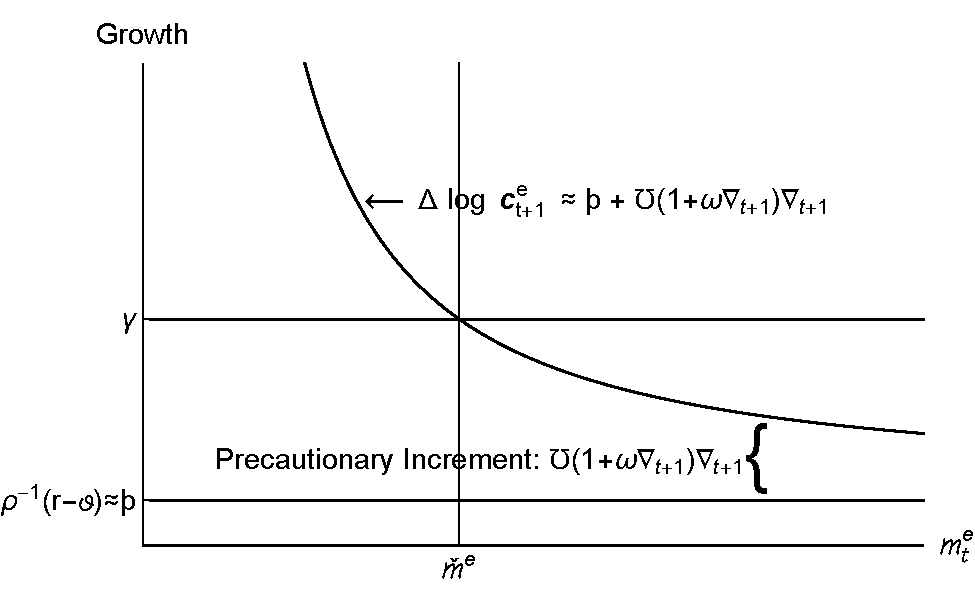
\includegraphics[width=6in]{../Figures/TractableBufferStockGrowthA}
\end{figure}

Next, note that the point where the consumption growth locus
meets the income growth line is labelled $\mTarg^{\null}$.  This is
because the place where consumption growth is equal to income
growth is at the target value of $\mRatE$.


\opt{MarginNotes}{\marginpar{\tiny $\mTarg^{\null}$ is point where impatience = prudence.}}

\subsubsection{Summing Up the Intuition}
We are finally in position to get an intuitive understanding of how the
model works, and why there is a target wealth ratio.  On the one hand,
consumers are growth-impatient.  This prevents their wealth-to-income ratio
from heading off to infinity.  On the other hand, consumers have
a precautionary motive that intensifies more and more as the level of
wealth gets lower and lower.  At some point the precautionary motive
gets strong enough to counterbalance impatience.  The point where impatience matches prudence defines the
target wealth-to-income ratio.


\begin{figure}
\caption{Effect of An Increase In $\rfree$}
\includegraphics[width=6in]{../Figures/TractableBufferStockGrowthB}
\label{fig:GrowthB}
\end{figure}

Now consider the results of increasing the interest rate to
$\grave{\rfree}>\rfree$, depicted in figure~\ref{fig:GrowthB}.  Obviously the perfect foresight consumption
growth locus will shift up, to $\CRRA^{-1}(\grave{\rfree}-\timeRate)$,
inducing a corresponding increase in the expected consumption growth
locus.  But we have not changed the expected growth rate of income.
It is clear from the figure, therefore, that the new target level of
cash-on-hand $\grave{\check{\mRat}}^{e}$ will be greater than the original target.
That is, an increase in the interest rate increases the target level
of wealth, as would be expected on intuitive grounds.

The next exercise is an increase in the risk of unemployment $\urate.$
The principal effect we are interested in is the upward shift in the expected
consumption growth locus to $\Delta \grave{\cLev}_{t+1}$.  If the
household starts at the original target level of resources
$\grave{m}$, the size of the upward shift at that point is captured by the
arrow orginating at $\{\check{m},\pGro\}$.  

In the absence of other consequences of the rise in $\urate$, the
effect on the target level of $\mRat$ would be unambiguously positive.
However, recall our adjustment to the growth rate conditional upon
employment, \eqref{eq:meanPreserve}; this induces the shift in the
income growth locus to $\grave{\pGro}$ which has an offsetting effect
on the target $\mRat$ ratio.  Under our benchmark parameter values,
the target value of $\mRat$ is higher than before the increase in risk
even after accounting for the effect of higher $\pGro$, but in
principle it is possible for the $\pGro$ effect to dominate the direct
effect.  Note, however, that even if the target value of $\mRat$ is
lower, it is possible that the {\it saving rate} will be higher; this
is possible because the faster rate of $\pGro$ makes a given saving
rate translate into a lower ratio of wealth to income.  In any case,
the most useful calibrations of the model are those for
which an increase in uncertainty results in either an increase in the
saving rate or an increase in the target ratio of resources to
permanent income.  This is partly because our intent is to use the
model to illustate the general features of precautionary behavior,
including the qualitative effects of an increase in the magnitude of
transitory shocks, which unambiguously increase both target $\mRat$
and saving rates.

\begin{figure}
\caption{Effect of an Increase in $\urate$}
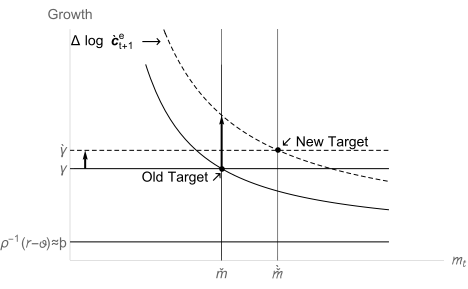
\includegraphics[width=6in]{../Figures/cGroIncreaseMhoPlot}
\label{fig:cGroIncreaseMhoPlot}
\end{figure}

\subsubsection{Death to the Log-Linearized Consumption Euler Equation!}

Figures~\ref{fig:GrowthA} and \ref{fig:GrowthB} show that, so long as
consumers are impatient, the steady state growth rate of consumption
will be equal to the steady-state growth rate of income,
\begin{equation}\begin{gathered}\begin{aligned}
        \Delta \log \cLevBF^{e}_{t+1} & =  \pGro. \label{eq:ceqg}
\end{aligned}\end{gathered}\end{equation}

Yet the approximate Euler equation for consumption growth, \eqref{eq:cLevGro}, does 
not contain any term explicitly involving income growth; in the logarithmic utility
case, for example, the expression is
\begin{equation}\begin{gathered}\begin{aligned}
         \Delta \log \cLevBF^{e}_{t+1} & \approx  \CRRA^{-1}(\rfree-\timeRate) +  \urate \nabla _{t+1}. \label{eq:cdelapprox2}
\end{aligned}\end{gathered}\end{equation}

How can we reconcile these two expressions for consumption growth?
Only by realizing that the size of the precautionary term $\urate
\nabla_{t+1}$ is {\it endogenous}: It depends on $\pGro$.  Indeed, we
can solve \eqref{eq:ceqg} and \eqref{eq:cdelapprox2} to determine that
in steady-state we must have \opt{MarginNotes}{\marginpar{\tiny Point
    out the SS $\urate \nabla$ on \ref{fig:GrowthB}.}}
\begin{equation}\begin{gathered}\begin{aligned}
        \urate \check{\nabla} & \approx  \pGro - \CRRA^{-1}(\rfree-\timeRate). \label{eq:prectermSS}
\end{aligned}\end{gathered}\end{equation}

We can use this equation to understand the relationship between
parameters and steady-state levels of wealth, by noting that
$\nabla_{t+1}(\mRatE_{t})$ is a downward-sloping function of
$\mRatE_{t}$ (see figure~\ref{fig:GrowthA} again).  This is because at
low levels of current wealth, much of the spending of employed
consumers is financed by their current income.  If they lose that
income, they will have no choice but to cut consumption drastically; this is
reflected in a large value of $\nabla_{t+1}$.

For example, an increase in the growth rate of income implies that the
RHS of equation \eqref{eq:prectermSS} increases.  The new target level of
$\mTarg^{\null}$ must be lower, because lower wealth induces greater consumption risk and a corresponding increase in the LHS of \eqref{eq:prectermSS}.  This is how the human wealth effect works in this framework:
Consumers who anticipate faster income growth will hold less market wealth.

The fact that consumption growth equals income growth in the
steady-state poses major problems for empirical attempts to estimate
the Euler equation.  To see why, suppose we had a collection of
countries indexed by $i$, identical in all respects except that
they have different interest rates $\rfree_{i}$.
Then in the spirit of \cite{hallSubstitution}, one might be
tempted to estimate an equation:
\begin{equation}\begin{gathered}\begin{aligned}
        \Delta \log \cLev_{i} & =  \eta_{0} + \eta_{1} \rfree_{i}+\epsilon_{i},
\end{aligned}\end{gathered}\end{equation}
and to interpret the coefficient estimate on $\rfree_{i}$ as an indication
of the value of $\CRRA^{-1}$.

But suppose that all of these countries contained impatient consumers
and were in their steady-states where $\Delta \log \cLev_{i} = \pGro_{i}$.
Suppose further
that all countries had {\it the same} steady-state income growth rate and
unemployment rate.\footnote{The key point holds even if countries have different
growth rates, but is easiest to understand if growth rates are identical.}
Then the regression equation would return the estimates
\begin{equation}\begin{gathered}\begin{aligned}
        \eta_{0} & =  \pGro  \\
        \eta_{1} & =  0.
\end{aligned}\end{gathered}\end{equation}

The econometric problem here is that there is an {\it omitted
variable} from the regression specification, the $\urate \nabla$ term, which is (perfectly) correlated with the included
variable $\rfree_{i}$.  Thus, Euler equation estimation cannot be expected to
return an unbiased estimate of $\CRRA^{-1}$.  For much more on this
problem, see \cite{carroll:death}.  For empirical evidence
that the problem is important in macroeconomic practice, see \cite{ParkerPrestonPrecaution}.

\subsubsection{A Final Experiment}
We now consider a final experiment: A decrease in the time preference
rate.  To reduce clutter, we drop the $\Delta \cE_{t+1}=0$ locus from the 
phase diagram from Figure~\ref{fig:PhaseDiag}, and everywhere drop $e$ the superscripts.  
(In exam questions, a figure like this might be referred to as the `simplified consumption phase diagram' or just
`the consumption diagram').

Figure~\ref{fig:DecreaseTheta} depicts the effect on the 
employed consumer's spending by
showing each successive point in time as a dot.  
Starting at time 0 from the steady-state level of consumption, the
decrease in the future discounting rate (an increase in patience) causes
an instantaneous drop in the level of consumption.  Starting from this diminished 
base, consumption growth is subsequently faster than before the drop in $\timeRate$.\footnote{We could also analyze the effects on growth, but the
  results would be essentially the same as in preceding figure
  analyzing the effect of an increase the interest rate.}

Eventually consumption approaches its new, higher equilibrium ratio
to permanent income at a new, higher level of equilibrium $\mRatE$.  This
higher level of consumption is financed in the long run by the higher
interest income earned on the higher level of wealth.

Note again, however, that equilibrium steady-state 
consumption growth is still equal to the growth rate of income (this follows
from the fact that there is a steady-state {\it level} for the {\it
  ratio} of consumption to income, $c$).  This means that the higher
level of wealth in equilibrium ends up being precisely enough to
reduce the precautionary term by an amount that exactly offsets the
fact that the $-\CRRA^{-1}\timeRate$ term in the Euler equation is now
smaller.

The final figures depict the time paths of consumption, market wealth,
and the marginal propensity to consume $\MPCFunc(\mRat)$ following the
decline in $\timeRate$.  These are implicit in the phase diagram
analysis, but the dots in these two new diagrams are spread out evenly
over time to give a sense of the time scale over which the model
adjusts toward the steady state.

\begin{figure}
\caption{Effect of Lower $\timeRate$ On Consumption Function}
\includegraphics[width=6in]{../Figures/PhaseDiagramDecreaseThetaPlot}
\label{fig:DecreaseTheta}
\end{figure}

\begin{figure}
\caption{Path of ${\cRat}^{e}$ Before and After $\timeRate$ Decline}
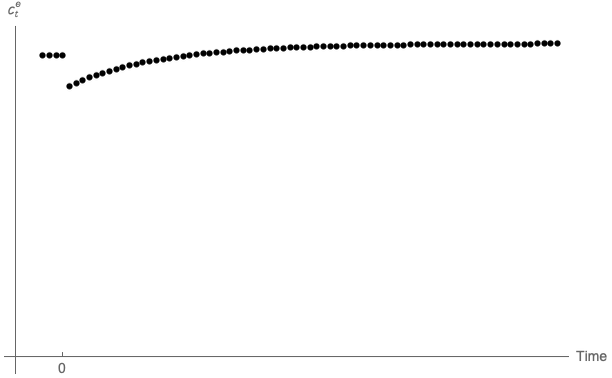
\includegraphics[width=6in]{../Figures/cPathAfterThetaDrop}
\label{fig:cPathAfterThetaDrop}
\end{figure}

\begin{figure}
\caption{Path of $\mRatE$ Before and After $\timeRate$ Decline}
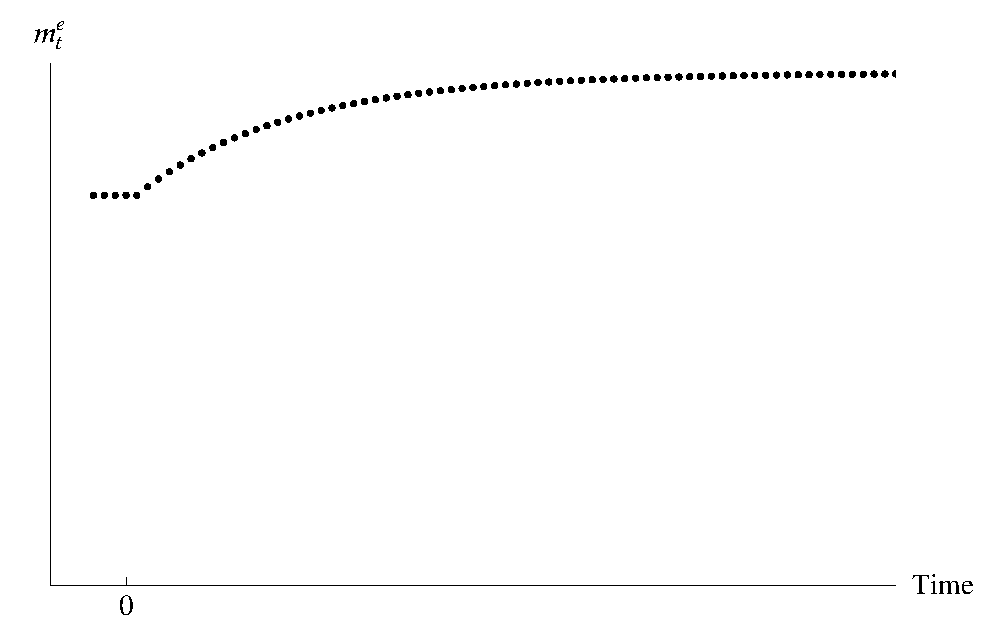
\includegraphics[width=6in]{../Figures/mPathAfterThetaDrop}
\label{fig:mPathAfterThetaDrop}
\end{figure}


\begin{figure}
\caption{Marginal Propensity to Consume $\MPC_{t}$ Before and After $\timeRate$ Decline}
\medskip
\includegraphics[width=6in]{../Figures/MPCPathAfterThetaDrop}
\label{fig:MPCPathAfterThetaDrop}
\end{figure}

\section{A Macroeconomic Interpretation}

Loosely following~\cite{cjSOE} (with some simplifications), this section extends the model to analyze macroeconomic dynamics in a
small open economy with a large number of individuals, where the
population statistics reflect the fulfillment of individual consumers'
{\it ex ante} expectations; for example, exactly proportion $\urate$
of households who are employed in period $t$ become `unemployed' before
$t+1$, so that the aggregate labor supply of the `active' (still employed) members of a generation
evolves according to
\begin{equation}\begin{gathered}\begin{aligned}
  \PopLev_{t+1,t} & =  \erate \PopLev_{t,t}
,
\end{aligned}\end{gathered}\end{equation}
where the first subscript denotes the date being examined and the second denotes
the period of birth of the generation being examined.

We make strong assumptions that permit straightforward aggregation. The first such assumption is that newly unemployed households immediately migrate out of the
country (think of British retirees moving to southern
Spain).\footnote{The qualitative story is not changed if the unemployed stay at home and live off their savings; since they have a simple linear
  decision rule (they spend a constant proportion of their resources),
  accounting for their behavior is straightforward but
  complicates the exposition without adding much substance.  See \cite{cjSOE} for a model that incorporates a stay-at-home unemployed population.}
This means that macroeconomic variables will reflect only the circumstances of 
employed consumers, rather than a blend of the employed and the unemployed.

Each person is part of a single `generation' of households born at the
same time, and every new generation is larger by the factor $\EmpGro$
than the newborn generation in the previous period:
\begin{equation}\begin{gathered}\begin{aligned}
  \PopLev_{t+1,t+1} & =  \EmpGro \PopLev_{t,t}
.
\end{aligned}\end{gathered}\end{equation}

We assume that total production by the (surviving) members of a generation grows by
the factor $\WGro$ every period.  If total production is to grow
despite a shrinking number of surviving members of the generation, 
production {\it per active capita} must grow by $\WGro/\erate$ as per \eqref{eq:meanPreserve}.

Consider the economy in some period 0 in which the size of the newborn population
and the wage rate have been normalized to $\PopLev_{0,0} = \Wage_{0} = 1$.  If the economy
has existed for $-\tThen$ periods (where $\tThen$ is a negative number, indicating that the economy was created before period 0), the ratio of the total population to the population
of newborns will be 
\begin{equation}\begin{gathered}\begin{aligned}
  1 + (\erate/\EmpGro)+ (\erate/\EmpGro)^{2}+ ... +(\erate/\EmpGro)^{-\tThen} & =  \left(\frac{1-(\erate/\EmpGro)^{-\tThen+1}}{1-(\erate/\EmpGro)}\right)
\end{aligned}\end{gathered}\end{equation}
whose limit is a finite number so long as $\erate/\EmpGro < 1$, which we require.

Relative to the labor income of period 0's newborn cohort ($\PopLev_{0,0} \Wage_{0} = 1$),
the total labor income in period 0 of the generation born in period $-1$ is $\EmpGro^{-1}$; the sum of the incomes of all of the two-period-old individuals is $\EmpGro^{-2}$, and so on; total labor income for all generations in the economy in period 0 is
\begin{equation}\begin{gathered}\begin{aligned}
  1 + \EmpGro^{-1}+ \EmpGro^{-2}+ ...+\EmpGro^{\tThen} & =  \left(\frac{1-(\EmpGro^{-1})^{-\tThen+1}}{1-\EmpGro^{-1}}\right) \label{eq:LabIncTot}
,
\end{aligned}\end{gathered}\end{equation}
which is finite so long as either population growth is positive $\EmpGro>1$ (which 
we will assume) or 
the economy has existed for a finite period of time ($\tThen > -\infty$).  
In either case, the {\it proportion} of aggregate income accounted for by a generation
born at any specific moment declines toward zero as time passes (old generations never die,
they just fade away).

In the balanced growth equilibrium, the growth factor for aggregate population
will therefore be $\EmpGro$ and output per capita will increase by $\WGro$ per period.  Total
labor income therefore grows by $\EmpGro \WGro.$


\subsection{Stakes}

We now examine this model under two assumptions about the initial
`stake' of newborns in the economy.  (We use `stake' to designate a
transfer received by newborns).  This is explicitly {\it not} an
inheritance, as we have assumed that individuals have no bequest
motive and newborns are unrelated to anyone in the existing
population.  Our motivation is to make the model more tractable,
rather than to represent an important feature of the real world; we
later perform simulations designed to show that the characteristics of
the model with no `stake' are qualitatively and quantitatively similar
to those of the more tractable model with the `stake' that makes the
model tractable.

\subsubsection{A `Stake' That Yields a Representative Agent}

We first consider a version of the model in which an exogenous
redistribution program guarantees that the behavior of employed households can 
be understood by analyzing the actions of a ``representative employed agent.''  

If a benevolent source outside the economy were to provide every newborn with an initial
transfer upon birth of size $\bTarg^{\null}$, then the newborn's total monetary resources 
would be
\begin{equation*}\begin{gathered}\begin{aligned}
  \mRatE_{t,t} & =  \bTarg^{\null} + 1
\\ & =  \mTarg^{\null} 
.
\end{aligned}\end{gathered}\end{equation*}

Thus, per-capita market resources for members of the newborn generation
would be exactly equal to the target level of market resources for a
person anticipating the future path of labor income that the members of the newborn
generation actually anticipate (which is the same as the future path
anticipated by all other generations as well).

If such a transfer policy had been in place forever, the economy at every 
point in time would consist of employed households whose consumption had 
been equal to its steady-state value ${\cRat}^{e}$ for their whole lives.  That is, every 
individual agent in this economy would be identical in their {\it ratio} of consumption,
market resources, etc.\ to permanent labor income.  
The behavior of any individual would therefore be fully captured by the behavior
of a representative employed agent.\footnote{The {\it level} of permanent 
labor income will differ for different households, depending on their age
and accumulated wage seniority; the circumstances of individuals are identical
only after their problem has been normalized by their varying levels of permanent 
labor income.}

The foregoing scenario assumed that the `stake' is provided by a mysterious
`benevolent source outside the economy.'  Fortunately, there is an
easy way to eliminate this problematic assumption: Assume that the
stakes are financed by a wage tax.

The size of the required tax rate is calculated as follows.  The total size
of the resources transferred to the newborn generation must be
\begin{equation}\begin{gathered}\begin{aligned}
  \hat{\bRat}^{e}_{t,t} & =  \hat{\bRat}^{\null} \PopLev_{t,t} \hat{\Wage}_{t}
\end{aligned}\end{gathered}\end{equation}
where
\begin{equation}\begin{gathered}\begin{aligned}
  \hat{\Wage}_{t} & =  \underbrace{\left(1-\Tax \right)}_{\equiv \TaxFree}\Wage_{t}
\end{aligned}\end{gathered}\end{equation}
is the after-tax wage rate for the economy as a whole (and $\hat{b}^{\null}$ is the steady state target ratio of bank balances to after-tax wages).

From \eqref{eq:LabIncTot}, the ratio of total aggregate labor income 
to the labor income of the newborn generation is 
\begin{equation}\begin{gathered}\begin{aligned}
  \left(\frac{1}{1-\EmpGro^{-1}}\right)
\end{aligned}\end{gathered}\end{equation}
so the aggregate wage tax rate required to finance a `stake' of size $\hat{b}^{\null}$ for
newborns is given by 
\begin{equation}\begin{gathered}\begin{aligned}
  \hat{b}^{\null} & =    \left(\frac{\Tax}{1-\EmpGro^{-1}}\right)
\\ \Tax & =  (1-\EmpGro^{-1})\hat{b}^{\null}
.
\end{aligned}\end{gathered}\end{equation}

Note, however, that in an economy where this tax has existed forever, the consequence
of the tax is effectively just a permanent reduction in after-tax labor income by proportion $\TaxFree$, compared to its value in the absence of the tax.  
Given the homotheticity of the model, a permanent rescaling by a constant 
factor leaves the scaled version of the individual's problem (and its solution)
unchanged.  Thus we can conclude not only that a representative agent exists
in this economy, but that the steady-state characteristics of the 
representative agent's problem are identical (in ratio form) to the 
characteristics of the unrescaled individual's problem; that is, 
$\hat{\cFunc}(\mRat) = \cFunc^{e}(\mRat)$, $\hat{b}^{\null} = \bTarg^{\null}$, and so on.  

Matters are not much more complicated outside the balanced growth
steady state, so long as we assume that the government always
transfers the amount $\hat{b}^{\null}$ to newborn households, financed by
the tax $\Tax$ derived above.  Consider, for example, an economy that
was in steady-state equilibrium leading up to period $\tNow$, and at
the beginning of $\tNow$ there is a sudden realization that future
growth rates will be higher than those anticipated and experienced in
the past: $\WGro^{\prime} > \WGro$ after $\tNow$.  Since expected
growth rates affect $\bTarg^{\null}$, the tax rate must be immediately and
permanently changed so that the generations born after $\tNow-1$
receive a `stake' of the proper new size.  This change in $\Tax$ has
two consequences for the generations that survive from periods prior
to $\tNow$.  Under the old tax rate, they would have experienced
$\bE_{t} = \bLevBF_{t}/\TaxFree\Wage_{t} = \bTarg^{\null}$; the change in
expectations has no effect on $\bLevBF_{t}$ or $\Wage_{t}$ but changes
the tax rate to $\grave{\Tax}$.  Thus these households will have an
actual resource ratio that differs from its new target value, $\bE_{t}
\neq \Alt{\bTarg}^{\null}$, both because the after-tax income scaling factor
has changed and because the target ratio has changed from $\bTarg^{\null}$
to $\Alt{\bTarg}^{\null}$.

However, if we started out in steady-state, the {\it ratio} problem of every
member of the continuing-employed population is identical to that of every 
other such household (though, again, their masses differ depending on age, etc); as a result, the dynamics of the economy are fully captured
by keeping track of the relative weights in the economy of the (gradually diminishing) `representative shocked agent' and the (gradually increasing) `representative new agent' 
whose behavior is locked at its steady-state value.\footnote{
If the economy has experienced multiple shocks, it will be necessary to
retain a complete history of the shocks in order to compute the properly 
population-weighted dynamics.  This is not too hard to do, if we start with
the assumption that the economy started at its balanced growth equilibrium before the shocks began to arrive.}

Figure~\ref{fig:SOEStakescPathAfterThetaDropPlot} illustrates the
dynamics in this economy using an experiment identical to one explored
above for the individual's problem: In period 0 there is a one-off
decline in the future discounting rate (assuming the economy was in
steady state before period 0).  In the previous model, each individual
consumer's consumption function shifted down, and consumption
experienced a discrete jump downward, because the agent became more
impatient.  Here, there is a modest further effect: With
more-patient consumers, the tax rate that the government sets to finance a transfer
of $\bTarg^{\null}$ to the newborns must be larger (so that the ratio of initial assets to
after-tax income is smaller).  Qualitatively, the
dynamics are indistinguishable from the individual consumer's dynamics
obtainable without working through the extra complication involved in
accounting for the `stakes.'

\begin{figure}
\caption{Aggregate $c$ in PE/SOE Economy Before and After $\timeRate$ Decline}
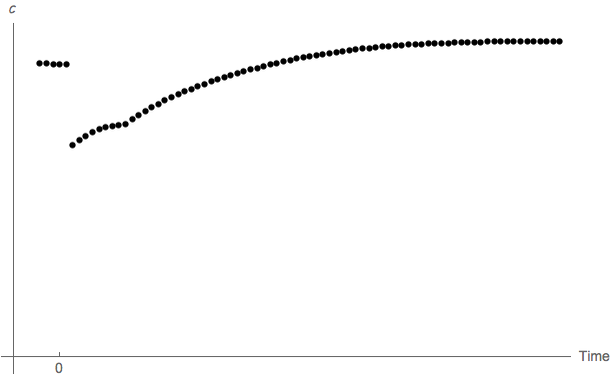
\includegraphics[width=6in]{../Figures/SOEStakescPathAfterThetaDropPlot}
\label{fig:SOEStakescPathAfterThetaDropPlot}
\end{figure}

\subsubsection{No Stake}

The polar alternative to assuming that newborns get a `stake' is to
assume that newborns enter the economy with zero assets.  Analysis of
this version of the model must be performed using simulation methods,
because households of different ages will have different levels of
assets.  (With a concave and nonanalytical consumption function,
analytical aggregation cannot be performed.)

Our simulation procedure assumes that at date 0 the economy has existed forever (so 
that the age distribution of relative populations and productivities are at their steady-state values), but saving has been impossible prior to
period 0.\footnote{In periods before 0, unemployment presumably would have 
meant immediate death by starvation; we think of this more as a starting point
for the simulations than as a realistic description of a plausible economy.}
With everyone's $\bE_{t}=0$, the ratio of market resources to permanent
labor income is the same for all individuals:
\begin{equation}\begin{gathered}\begin{aligned}
  \mRatE_{0,\tThen} & =  1
.
\end{aligned}\end{gathered}\end{equation}
The consumption ratio in period 0 is therefore $\cFunc(1)$ for every
household (regardless of age), while the
level of total labor income for a generation that is $-\tThen$ periods old is $\erate^{\tThen}$.\footnote{The absolute level of wages will have
grown by $\WGro/\erate$ per period for these households since their birth, but we have normalized by the level of wages
for period-0 newborns, which cancels the $\WGro$ from the expression.}  The population of
such workers is $(\erate/\EmpGro)^{-\tThen}$, so aggregate consumption will
be given by the per-capita consumption ratio, multiplied by the
per-capita level of permanent income, multiplied by the population of
workers still alive:
\begin{equation}\begin{gathered}\begin{aligned}
  \cLev_{0} & =  \sum_{\tThen=0}^{-\infty} \cFunc(1) \erate^{\tThen} (\erate/\EmpGro)^{-\tThen}
\\ & =  \cFunc(1) \sum_{\tThen=0}^{-\infty}  \EmpGro^{\tThen}
\\ & =  \cFunc(1) \left(\frac{1}{1-\EmpGro^{-1}}\right)
.
\end{aligned}\end{gathered}\end{equation}

The longer a generation lives, the more time it will have had to save toward
its target level of wealth; but newborns always begin life with no assets.  After period 0, therefore, age-heterogeneity in assets and consumption ratios creeps into the population.

The foregoing discussion contains (in some cases implicitly) all the
assumptions necessary to conduct a simulation of this economy.
Figure~\ref{fig:SOENoStakescPath} shows the path of the ratio $\cLev_{t}/\Wage_{t}\PopLev_{t}$ starting from
period 0 for an economy under our benchmark parameterization that generated
our earlier figures.  The
only extra parameter required beyond those used before is $\EmpGro$; we choose $\EmpGro=1.01$ corresponding
roughly to the postwar population growth rate in the United States.

\begin{figure}
\caption{Path of Aggregate $c$ in Stakeless PE/SOE Economy From Date 0}
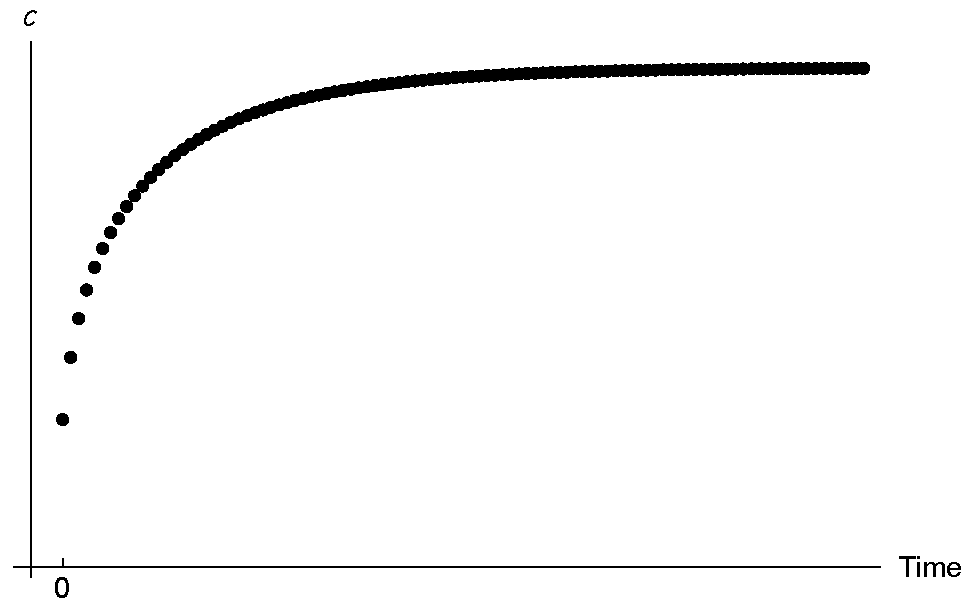
\includegraphics[width=6in]{../Figures/SOENoStakescPath}
\label{fig:SOENoStakescPath}
\end{figure}



\label{sec:PFwhenFHWfails}
\pagebreak\appendix
\centerline\textbf{\LARGE Appendix}\medskip

\setcounter{section}{0}

\section{Approximate Formula for Consumption Growth}\label{sec:CGroApprox}

Using from \MathFactsList ~the second-order and then the first-order
Taylor approximations  \TaylorTwo $(1+\epsilon)^{\zeta} \approx 1 + \zeta \epsilon +
(1/2)\zeta(\zeta-1) \epsilon^{2}$ and then \TaylorOne $(1+\epsilon)^{\zeta} \approx 1 + \zeta \epsilon$, the expression in braces
in \eqref{eq:cedel} can be rewritten
\begin{equation}\begin{gathered}\begin{aligned}
        \left\{1+\urate\left[\left(\frac{{\cRat}^{e}_{t+1}}{\cU_{t+1}}\right)^{\CRRA}-1\right]\right\}^{1/\CRRA} & =  \left\{1+\urate\left[\left(\frac{\cU_{t+1}+{\cRat}^{e}_{t+1}-\cU_{t+1}}{\cU_{t+1}}\right)^{\CRRA}-1\right]\right\}^{1/\CRRA} \notag
\\      & =  \left\{1+\urate\left[\left(1+\nabla _{t+1}\right)^{\CRRA}-1\right]\right\}^{1/\CRRA} \notag
\\      & \approx       \left\{1+\urate\left[1+\CRRA \nabla _{t+1}+ \CRRA (\nabla _{t+1})^{2}\prudEx-1\right]\right\}^{1/\CRRA} \notag 
\\ & =          \left\{1+ \CRRA \urate (\nabla _{t+1}+ (\nabla _{t+1})^{2}\prudEx)\right\}^{1/\CRRA} \notag
\\ & \approx  1+ \urate  \left(1+\nabla _{t+1}\prudEx\right)\nabla _{t+1}, \notag
\end{aligned}\end{gathered}\end{equation}
which leads directly to \eqref{eq:cedelapprox} in the main text.


\section{Conditions for a Target to Exist}\label{sec:mTargExists}

\subsection{Using the Phase Diagram Loci} 
 
At a steady-state value of $\mRatE$, both $\dcEqZero$ and $\dmEqZero$ hold (equations \eqref{eq:cDelEqZero} and \eqref{eq:mDelEqZero}); for convenience defining $\mu = \Rnorm \MPCU \straight + 1$, 
\begin{equation}\begin{gathered}\begin{aligned}
  0 = \overbrace{\left(\frac{\mu-1}{\mu}\right) \mRatE}^{\Delta {\cRat}^{e} } & =  \overbrace{\left(\frac{\Rnorm-1}{\Rnorm}\right)\mRatE + \Rnorm^{-1}}^{\Delta \mRatE} = 0.
\end{aligned}\end{gathered}\end{equation}
But since $\Rnorm^{-1}$ is a positive number, at $\mRatE=0$ the $\dmEqZero$ locus's value is $\Rnorm^{-1}$ while the value of the $\dcEqZero$ locus is zero, the two loci can intersect for a positive $\mRatE$ only if the slope of the $\dcEqZero$ locus is greater:\footnote{We also need $\mu$ to be nonnegative.}
\begin{equation}\begin{gathered}\begin{aligned}
  \left(\frac{\mu-1}{\mu}\right) & >  \left(\frac{\Rnorm-1}{\Rnorm}\right) \label{eq:cDelEq0SlopeCond}
\end{aligned}\end{gathered}\end{equation}
which is equivalent to 
\begin{equation}\begin{gathered}\begin{aligned}
  \overbrace{\Rnorm \MPCU \straight}^{= \mu-1} & >   \Rnorm-1  \label{eq:cDelEq0SlopeCondAlt}
\end{aligned}\end{gathered}\end{equation}
where the LHS is (proportional to) the slope of $\dcEqZero$ and the RHS is (proportional to) the slope of $\dmEqZero$.

For any fixed $\urate$ and $\WGro$ and $\Rfree$ we can find some $\alpha$ for which $\WGro = \Rfree (1-\alpha \urate)$, and using this $\alpha$ it turns out to be useful to rewrite
\begin{equation}\begin{gathered}\begin{aligned}
  \Rnorm^{-1} & =  \PGro/\Rfree
\\ & =  \WGro/\Rfree(1-\urate)
\\ & =  \Rfree(1-\alpha \urate)/\Rfree(1-\urate)
\\ & =  (1-\alpha \urate + \urate - \urate)/(1-\urate)
\\ & =  (1-\urate+(1-\alpha) \urate)/(1-\urate)
\\ & =  1+(1-\alpha)\urate/(1-\urate) \label{eq:RnormFromAlpha}
.
\end{aligned}\end{gathered}\end{equation}

Note for future use that \eqref{eq:RnormFromAlpha} implies that whenever $\alpha \leq 1$, the \FHWCPGro~fails (`human wealth is infinite') because $\Rnorm^{-1} > 1 \Rightarrow \Rfree/\PGro = \Rnorm < 1 \Rightarrow \Rfree < \PGro$.  

Multiplying both sides of \eqref{eq:cDelEq0SlopeCondAlt} by $\Rnorm^{-1}$ then substituting the expression for $\Rnorm^{-1}$ from \eqref{eq:RnormFromAlpha} gives
\begin{equation}\begin{gathered}\begin{aligned}
  1- \Rnorm^{-1} & <  \MPCU \straight
\\ - (1-\alpha)\urate/(1-\urate) & <  \MPCU \straight \label{eq:alphaReq}
\end{aligned}\end{gathered}\end{equation}

\subsection{A Target Always Exists When Human Wealth Is Infinite}

Since $0 < \urate < 1$ and $\MPCU>0$ (as guaranteed by the RIC), \eqref{eq:alphaReq} is satisfied whenever the \FHWCPGro~fails ($\alpha \leq 1$) and $\straight > 0$.
We now show that under these conditions, $(1+\varpi)^{1/\CRRA}=\straight>0$.  

$\straight$ from \eqref{eq:straightDef} is:
\begin{equation}\begin{gathered}\begin{aligned}
  \straight & =  \left(1+\overbrace{\urate^{-1}(\GPFacRaw^{-\CRRA}-1)}^{\equiv \varpi}\right)^{1/\CRRA}
\end{aligned}\end{gathered}\end{equation}
but note that 
\begin{equation}\begin{gathered}\begin{aligned}
  \GPFacRaw & =  \PatR \overbrace{(\Rfree/\PGro)}^{=\Rnorm}
\end{aligned}\end{gathered}\end{equation}
and in the case where $\alpha=1$, $\Rnorm$ must also be 1, implying that $\GPFacRaw = \PatR < 1$ (the RIC) so that $\GPFacRaw^{-\CRRA} > 1$ and so $\varpi > 0$ and hence $\straight > 1 > 0$.  The other interesting case is when $\alpha=0$ so that $\WGro=\Rfree$ and $\Rnorm=\Rfree/\PGro=\Rfree(1-\urate)/\WGro=(1-\urate)<1$.  In this case $\GPFacRaw < \PatR$ and so $\GPFacRaw^{-\CRRA} > \PatR^{-\CRRA} > 1$ and so $\varpi$ is even more positive so that $\straight$ is even more strongly $>0$.  Similar logic holds for any $\alpha \leq 1$.  

Thus, we can conclude that, when human wealth is infinite (that is, if $\alpha \leq 1$), a target $\Target{\mRat}^{e}$ will exist.  

\subsection{Conditions Under Which a Target Exists When Human Wealth is Finite}

In the case where human wealth is finite ($\alpha > 1$), we need the RHS of \eqref{eq:alphaReq} not merely to be positive, but to exceed a specific positive number, $(\alpha-1)\urate/(1-\urate)$:  
\begin{equation}\begin{gathered}\begin{aligned}
    \MPCU (1+\varpi)^{1/\CRRA} & >  (\alpha-1)\urate/(1-\urate)
\\   (1+\varpi)^{1/\CRRA} & >  \left(\frac{(\alpha-1)\urate}{\MPCU (1-\urate)}\right)
\\   (1+\varpi) & >  \left(\frac{(\alpha-1)\urate}{\MPCU (1-\urate)}\right)^{\CRRA}
\\  (\GPFacRaw^{-\CRRA}-1)\urate^{-1} = \varpi & >  \left(\frac{(\alpha-1)\urate}{\MPCU (1-\urate)}\right)^{\CRRA}-1
\\  (\GPFacRaw^{-\CRRA}-1) & >  \urate \left[\left(\frac{(\alpha-1)\urate}{\MPCU (1-\urate)}\right)^{\CRRA}-1\right]
\\  \GPFacRaw^{-\CRRA} & >  1  + \urate \left[\left(\frac{(\alpha-1)\urate}{\MPCU (1-\urate)}\right)^{\CRRA}-1\right]
\\  \GPFacRaw & <  \left\{1  + \urate \underbrace{\left[\left(\frac{(\alpha-1)\urate}{\MPCU (1-\urate)}\right)^{\CRRA}-1\right]}_{\equiv \chi} \right\}^{-1/\CRRA} \label{eq:GPFacRawReqForTarget}
%\\  \GPFacRaw & <  \left\{1  + \urate \left[\left(\frac{(\alpha-1)\urate-\MPCU (1-\urate)}{\MPCU (1-\urate)}\right)^{\CRRA}\right] \right\}^{-1/\CRRA}
%\\  \GPFacRaw & <  \left(\frac{1}{\MPCU (1-\urate)}\right)^{-1/\CRRA}\left\{\MPCU (1-\urate)  + \urate \left[\left((\alpha-1)\urate-\MPCU (1-\urate)\right)^{\CRRA}\right] \right\}^{-1/\CRRA} \notag
%\\  \GPFacRaw & <  \left(\MPCU (1-\urate)\right)^{1/\CRRA}\left\{\MPCU (1-\urate)  + \urate \left[\left((\alpha-1)\urate-\MPCU (1-\urate)\right)^{\CRRA}\right] \right\}^{-1/\CRRA} \notag
\end{aligned}\end{gathered}\end{equation}
and the boundary will be the point at which this expression holds with equality.  

An increase in impatience caused by an increase in the pure time preference rate $\timeRate$ (equivalently, a reduction in $\Discount$) has the effect of reducing growth-patience (the LHS of \eqref{eq:GPFacRawReqForTarget}) and of increasing the RHS.  This means that there will be some time preference rate sufficiently large (some $\Discount$ sufficiently small) to guarantee that the condition holds with equality.  Then \eqref{eq:GPFacRawReqForTarget} will always be satisfied by any $\Discount$ satisfying \providecommand{\DiscountMaxGICWhenFHWCTBSHolds}{\ensuremath{\bar{\Discount}_{\text{FHW}}}}
\begin{equation}\begin{gathered}\begin{aligned}
  \Discount & <  \DiscountMaxGICWhenFHWCTBSHolds \label{eq:DiscountMaxGICWhenFHWCTBSHolds}
.\end{aligned}\end{gathered}\end{equation}


Since we have assumed the RIC (so that $\MPCU > 0$), as $\urate \downarrow 0$ or $\alpha \downarrow 1$, \eqref{eq:GPFacRawReqForTarget} asymptotes to the \GICPGro~for any given value of $\Discount$.  

The apparently harder case is when $\alpha>1$ and $\urate > 0$.  But note that we will have found $\DiscountMaxGICWhenFHWCTBSHolds$ if we can find the corresponding $\MPCU$ at which the first term in $\chi$ reaches 1:
\begin{equation}\begin{gathered}\begin{aligned}
    \left(\frac{(\alpha-1)\urate}{(1-\PatR) (1-\urate)}\right)^{\CRRA} & =  1
\\  \left(\frac{(\alpha-1)\urate}{(1-\PatR) (1-\urate)}\right) & =  1
\\  \left(\frac{(\alpha-1)\urate}{ (1-\urate)}\right) & =  1-\PatR
\\  1-\left(\frac{(\alpha-1)\urate}{ (1-\urate)}\right) & =  \PatR
\\                  \left[1-\left(\frac{(\alpha-1)\urate}{ (1-\urate)}\right)\right] & =  (\Rfree \Discount)^{1/\CRRA}/\Rfree
\\  \Rfree^{\CRRA}  \left[1-\left(\frac{(\alpha-1)\urate}{ (1-\urate)}\right)\right]^{\CRRA} & =  (\Rfree \Discount)
\\  \Rfree^{\CRRA-1}\left[1-\left(\frac{(\alpha-1)\urate}{ (1-\urate)}\right)\right]^{\CRRA} & =  \DiscountMaxGICWhenFHWCTBSHolds \label{eq:DiscountMaxGICWhenFHWCTBSHoldsAndGICPGroIsExactlySatisfied}
.\end{aligned}\end{gathered}\end{equation}

Somewhat miraculously, at this value of $\Discount$, because $\chi=0$, \eqref{eq:GPFacRawReqForTarget} holds with equality, which means that $\DiscountMaxGICWhenFHWCTBSHolds=\DiscountMaxGICPGro$.  This means that the \GICPGro~defines the definitive boundary condition:  A finite target $\mRatE$ exists so long as $\Discount < \DiscountMaxGICPGro = \PGro^{\CRRA}/\Rfree.$

\subsection{Solutions Exist Even When Growth Impatience Fails}

We have just demonstrated that satisfying the \GICPGro~condition is necessary and sufficient to guarantee existence of a target $\mTarg^{e}$.  But we suggested earlier that a weaker condition, the GIC-TBS, guarantees the existence of a well-defined consumption function.

This can be understood as follows.  Rewrite the requirement for existence of a target, \eqref{eq:cDelEq0SlopeCondAlt}, as 
\begin{equation}\begin{gathered}\begin{aligned}
  \MPCU (1+\varpi)^{1/\CRRA}+1 & >   \Rnorm  \label{eq:cDelEq0SlopeCondAltAlt}
,\end{aligned}\end{gathered}\end{equation}
or taking logs we have approximately 
\begin{equation}\begin{gathered}\begin{aligned}
  \MPCU (1+\varpi)^{1/\CRRA} & >   \rfree-\pGro \label{eq:cDelEq0SlopeCondLog}
.\end{aligned}\end{gathered}\end{equation}

The LHS captures the slope of the $\dcEqZero$ locus, which is $\MPCU$ modified by $\varpi$ whose difference from $\varpi=0$ captures the degree of growth (im)patience.\footnote{`Captures' does not mean `is equal to.'  Equation~\eqref{eq:cDelEq0SlopeCondAlt} provides the actual formula for the slope.}  The RHS captures the slope of the $\dmEqZero$ locus.  Recall that the inequality captures the fact that a target $\mTarg^{e}$ exists if these two loci intercept, which happens if the slope of $\dcEqZero$ exceeds that of $\dmEqZero$.

If the consumer is `growth patience poised' (that is, $\GPFacRaw = 1$), then $\varpi = 0$ and the slope of the $\dcEqZero$ locus is identical to the $\MPCU$ that characterizes the perfect foresight consumption function.  In this case \eqref{eq:cDelEq0SlopeCondLog} becomes
\begin{equation}\begin{gathered}\begin{aligned}
  \rfree-\CRRA^{-1}(\rfree-\timeRate) & >   \rfree-\pGro
\\ \pGro & >  \CRRA^{-1}(\rfree-\timeRate) \label{eq:patpGroLT0}
,\end{aligned}\end{gathered}\end{equation}
which is the (log version of) the \GICPGro.  The condition cannot hold both as an equality $\GPFacRaw=1$ (our starting assumption) and an inequality $\GPFacRaw < 1$ (the conclusion of \eqref{eq:patpGroLT0}).  This contradiction constitutes a proof that exactly at $\GPFacRaw=1$ a target does not exist.


As noted above, if the consumer is growth-impatient ($\GPFacRaw < 1$) then $\varpi > 0$ and the slope of $\dcEqZero$ is monotonically increased as the degree of growth-impatience increases (so that target $\Target{\mRat}^{e}$ is diminished).  

But if the consumer is growth-patient ($\GPFacRaw > 1$) then $\varpi < 0$ and the slope of $\dcEqZero$ is diminished (which reflects the fact that the greater the degree of patience, the lower will consumption be for any given $\mRatE$).\footnote{Note that if the \GICPGro~fails so that $\straight < 1$, the slope of the $\dcEqZero$ locus is shallower than the slope of the perfect foresight consumption function.  The fact that these two loci never intersect reflects the fact that the consumer will behave in such a way as to accumulate $\mRatE$ forever.}  The lower bound is defined by the point at which the degree of growth patience becomes so strong that the slope of $\dcEqZero$ reaches zero (when $\straight=0$; equivalently, $\varpi$ reaches -1).  This restricts the permissible degree of growth patience, because $\straight > 0$ requires (rewrite \eqref{eq:GICExistsSoln}):
\begin{equation}\begin{gathered}\begin{aligned}
  \left(\frac{(\Rfree \Discount (1-\urate))^{1/\CRRA}}{\WGro/(1-\urate)}\right) = \left(\frac{(\Rfree \Discount (1-\urate))^{1/\CRRA}}{\PGro}\right) & <  1
.\end{aligned}\end{gathered}\end{equation}

Expanding on a discussion in the main text, the numerator in the leftmost expression reflects the sense in which the unemployment risk acts in a manner similar to the effect of an extra degree of discounting (reflecting the fact that the relevant condition applies only so long as the consumer remains in employment -- a condition whose probability is $(1-\urate)$), while the denominator reflects the mechanical effect in which the relevant measure of growth is boosted by the adjustment that preserves human wealth.  Writing the perfect foresight version of the growth patience factor as $\Pat_{\WGro}$ (which is just the limit as $\urate \downarrow 0$), we can see that the expression on the LHS is just $\Pat_{\WGro}(1-\urate)^{1+1/\CRRA}$ which is smaller than $\Pat_{\WGro}$ because $\urate>0$ and $1+\CRRA^{-1} > 0$.  So, the GIC-TBS holds whenever the plain-vanilla \GICPGro~holds, but not vice-versa; there are parametric configurations in which a perfect-foresight consumer with income growth rate $\WGro$ would not satisfy the relevant \GICWGro~(so, their wealth-to-income ratio would go to infinity), but the same consumer faced the same human wealth but with an unemployment risk $\urate$ would have a finite target wealth-to-income ratio.  


The easiest way to understand all of this is graphically.  A notebook \cite{When-FHWC-Holds} (see references for details) in the code archive associated with these lecture notes shows how this works for alternative values of $\Discount.$


\section{The Exact Formula for Target $m$}\label{sec:mTargExact}

To simplify the expressions in the derivations below, we define $\zeta \equiv \Rnorm \MPCU \straight$ so that $\Rfree \MPCU \straight = \zeta \PGro$ and we drop the $e$ superscripts, allowing \eqref{eq:cDelEqZero} to be rewritten as 
\begin{equation}\begin{gathered}\begin{aligned}
  \cRat_{\tSS} & =  \left(\frac{\zeta }{1+\zeta}\right)\mRat .
\end{aligned}\end{gathered}\end{equation}

If a target value $\mTarg$ exists it will be at the point of intersection between the $\dcEqZero$ and the $\dmEqZero$ loci:
\begin{equation}\begin{gathered}\begin{aligned}
  \left(\frac{\zeta}{1+\zeta}\right)\mTarg^{\null} & =  (1-\Rnorm^{-1})\mTarg^{\null}+\Rnorm^{-1}
\\  \left(\Rnorm\frac{\zeta}{1+\zeta}\right)\mTarg^{\null} & =  (\Rnorm-1)\mTarg^{\null}+1
\\  \left(\Rnorm\left\{\frac{\zeta}{1+\zeta}-1\right\}+1\right)\mTarg^{\null} & =  1
\\  \left(\Rnorm\left\{\frac{\zeta-(1+\zeta)}{1+\zeta}\right\}+\frac{1+\zeta}{1+\zeta}\right)\mTarg^{\null} & =  1
\\  \left(\frac{1+\zeta-\Rnorm}{1+\zeta}\right)\mTarg^{\null} & =  1
\\  \mTarg^{\null} & =  \left(\frac{1+\zeta}{1+\zeta-\Rnorm}\right)
\\  \mTarg^{\null} & =  \left(\frac{1+\zeta+\Rnorm-\Rnorm}{1+\zeta-\Rnorm}\right)
\\ & =  1 + \left(\frac{\Rnorm}{1+\zeta-\Rnorm}\right)
\\ & =  1 + \left(\frac{\Rfree}{\PGro+\zeta\PGro-\Rfree}\right)  \label{eq:mTarget}
.
\end{aligned}\end{gathered}\end{equation}

A first point about this formula is suggested by the fact that
\begin{equation}\begin{gathered}\begin{aligned}
  \zeta\PGro & =  \Rfree \MPCU \left(1+\left(\frac{\GPFacRaw^{-\CRRA} - 1}{\urate}\right)\right)^{1/\CRRA}
\end{aligned}\end{gathered}\end{equation}
which is likely to increase as $\urate$ approaches zero.\footnote{`Likely' but not certain because of the fact that $\urate$ affects $\GPFacRaw$ as well as
  appearing in the denominator of \eqref{eq:mTarget}; however, for
  plausible calibrations the effect of the denominator predominates.}
Note that the limit as $\urate \rightarrow 0$ is infinity, which
implies that $\lim_{\urate \rightarrow
  0} \mTarg^{\null} = 1$.  This is precisely what would be expected from
this model in which consumers are impatient but self-constrained to
have $\mRatE > 1$:  As the risk gets infinitesimally small, the
amount by which target $\mRatE$ exceeds its minimum possible value shrinks to
zero.

We now show that the RIC and \GICPGro~ensure that the denominator of the fraction in \eqref{eq:mTarget} is positive: 
\begin{equation*}\begin{gathered}\begin{aligned}
\PGro + \zeta \PGro - \Rfree & =  \PGro + \Rfree \MPCU \straight - \Rfree
 \\& =  \PGro + \Rfree \left(1- \frac{(\Rfree \Discount)^{1/\rho}}{\Rfree}\right) \left(\frac{(\frac{(\Rfree\Discount)^{1/\CRRA}}{\PGro})^{-\CRRA}-1}{\urate}+1\right)^{1/\CRRA}-\Rfree
 \\& >   \PGro+\Rfree \left(1-\frac{(\Rfree\Discount)^{1/\rho}}{\Rfree}\right)
\left(\frac{(\frac{(\Rfree\Discount)^{1/\CRRA}}{\PGro})^{-\CRRA}-1}{1}+1\right)^{1/\CRRA}-\Rfree
 \\& =  \PGro+\Rfree\left(1-\frac{(\Rfree\Discount)^{1/\rho}}{\Rfree}\right)\frac{\PGro}{(\Rfree\Discount)^{1/\CRRA}}-\Rfree
 \\& =  \PGro+\Rfree \frac{\PGro}{(\Rfree\Discount)^{1/\CRRA}}- \PGro - \Rfree
 \\& =  \Rfree \left(\frac{\PGro}{(\Rfree\Discount)^{1/\CRRA}}-1\right)
 \\& >  0.
\end{aligned}\end{gathered}\end{equation*}

However, note that $\urate$ also affects $\PGro$; thus, the first inequality above does
not necessarily imply that the denominator is decreasing as $\urate$ moves from $0$ to $1$.


\section{Approximating Target $m$}

Now defining
\begin{equation}\begin{gathered}\begin{aligned}
  \aleph & =  \left(\frac{\GPFacRaw^{-\CRRA} - 1}{\urate}\right),
\end{aligned}\end{gathered}\end{equation}
under certain conditions we can obtain further insight into \eqref{eq:mTarget} using a judicious mix of first- and second-order Taylor expansions (along with $\MPCU = -\patr$):\footnote{See below for caveats.}
\begin{equation}\begin{gathered}\begin{aligned}
  \label{eq:zetaExp}
  \zeta\PGro & =  \Rfree \MPCU \left(1+\aleph\right)^{1/\CRRA}
\\ & \approx  -\Rfree \patr \left(1+\CRRA^{-1}\aleph+(\CRRA^{-1})(\CRRA^{-1}-1)(\aleph^{2}/2)\right)
\\ & =  -\Rfree \patr \left(1+\CRRA^{-1}\aleph\left\{1+\left(\frac{1-\CRRA}{\CRRA}\right)(\aleph/2)\right\}\right) %\label{eq:zetaTaylor2}
%\\ & \approx  - \Rfree \patr \left\{1+\CRRA^{-1}\left(\frac{(1+\patpGro)^{-\CRRA} - 1}{\urate}\right)\right\}
%\\ & \approx  - \Rfree \patr \left\{1+\CRRA^{-1}\left(\frac{1-\CRRA \patpGro- 1}{\urate}\right)\right\}
%\\ & \approx  - \Rfree \patr\left(1+\left(\frac{1}{\CRRA}\right)\frac{1-\CRRA\patpGro - 1}{\urate}\right)
%\\ & =  -\Rfree \patr \left\{1-(\patpGro/\urate)\left(1-(\CRRA+1)\patpGro/2\right)\right\}
.
\end{aligned}\end{gathered}\end{equation}

But
\begin{equation}\begin{gathered}\begin{aligned}
  \label{eq:hatpi}
  \aleph & =  \left(\frac{(1+\patpGro)^{-\CRRA}-1}{\urate}\right)
\\ & \approx  \left(\frac{1- \CRRA \patpGro-1}{\urate}\right)
\\ & \approx  -\left(\frac{\CRRA \patpGro}{\urate}\right)
\end{aligned}\end{gathered}\end{equation}
which is guaranteed to be positive by the \GICPGro, but which can take any value in the interval $(0,\infty)$.  Note, however, that the approximations above are valid only if $\aleph$ is `small' which requires that the degree of growth impatience be small relative to the size of the unemployment risk.  Thus, the formulae derived above (and used below) are reliable only in rather special circumstances, in particular when the consumer is only very slightly growth-impatient.\footnote{Other approximations are better for consumers who are highly impatient, relative to their unemployment risk; in this case a better approximation to \eqref{eq:zetaExp} is obtained by rewriting it as $\zeta\PGro = \Rfree \MPCU \aleph^{1/\CRRA} \left(\aleph^{-1}1+1\right)^{1/\CRRA}$ and approximating using $(1+\aleph^{-1})^{1/\CRRA} \approx 1 + \CRRA^{-1}\aleph^{-1}+\CRRA^{-1}(\CRRA^{-1}-1)\aleph^{-2}/2$.}  Under these circumstances, this approximation can be substituted into \eqref{eq:zetaExp} to obtain
\begin{equation}\begin{gathered}\begin{aligned}
  \zeta\PGro & \approx   -\Rfree \patr \left(1-(\patpGro/\urate)(1+(1-\CRRA)(-\patpGro/\urate)/2)\right)
\\ & \approx  \underbrace{-\Rfree \patr}_{>0} \left\{1\underbrace{-(\patpGro/\urate)}_{>0}\left(1+\underbrace{(1-\CRRA)}_{<0}\underbrace{(-\patpGro/\urate)}_{>0}/2\right)\right\} \label{eq:zetaGammaApprox}
.
\end{aligned}\end{gathered}\end{equation}
and inspired by~\cite{kimball:smallandlarge} defining a term related to the excess of prudence
over the logarithmic case,
\begin{equation}\begin{gathered}\begin{aligned}
  \prudEx & =  \left(\frac{\CRRA-1}{2}\right),
\end{aligned}\end{gathered}\end{equation}
\eqref{eq:mTarget} can be approximated by
\begin{equation}\begin{gathered}\begin{aligned}
 \mTarg^{\null} & \approx  1 + \left(\frac{1}{\PGro/\Rfree-\patr \left(1-(\patpGro/\urate)(1-(-\patpGro/\urate)\prudEx) \right)-1}\right)
\\ & \approx  1 + \left(\frac{1}{(\pGro-\rfree)+(-\patr) \left(1+(-\patpGro/\urate)(1-(-\patpGro/\urate)\prudEx)\right)}\right)
\label{eq:mTargetApprox}
\end{aligned}\end{gathered}\end{equation}
where negative signs have been preserved in front of the $\patr$ and $\patpGro$ terms as a reminder that
the \GICPGro~and the RIC imply these terms are themselves negative (so that $-\patr$ and $-\patpGro$ are positive).
{\it Ceteris paribus}, an increase in relative risk aversion $\CRRA$ will increase $\prudEx$ and thereby decrease the denominator of \eqref{eq:mTargetApprox}.  This suggests that
greater risk aversion will result in a larger target level of wealth.\footnote{``Suggests'' because
this derivation used some dubious approximations; the suggestion is verified, however, for
plausible numerical calibrations.}


The formula also provides insight about how the human wealth effect
works in equilibrium.  All else equal, the human wealth effect is captured
by the $(\pGro-\rfree)$ term in the denominator of \eqref{eq:mTargetApprox},
and it is obvious that a larger value of $\pGro$ will result in a smaller
target value for $m$.  But it is also clear that the size of the human wealth
effect will depend on the magnitude of the patience and prudence contributions
to the denominator, and that those terms can easily dominate the human wealth
effect.  This reduction in the human wealth effect is interesting because practitioners have known at least since
\cite{summersCapTax} that the human wealth effect is implausibly large in the
perfect foresight model.

For \eqref{eq:mTargetApprox} to make sense, we need
the denominator of the fraction to be a positive number;
defining
\begin{equation}\begin{gathered}\begin{aligned}
  \patpGrohat & =  \patpGro(1-(-\patpGro/\urate)\prudEx),
\end{aligned}\end{gathered}\end{equation}
this means that we need:
\begin{equation}\begin{gathered}\begin{aligned}
    (\pGro - \rfree) & >  \patr - \patr\patpGrohat/\urate
\\   & =  \left(\CRRA^{-1}(\rfree-\timeRate)-\rfree\right)-  \patr\patpGrohat/\urate
\\ \pGro & >  \CRRA^{-1}(\rfree-\timeRate)-  \patr\patpGrohat/\urate
%\\ 0 & >  \underbrace{\CRRA^{-1}(\rfree-\timeRate) - \pGro}_{<0} -  \patr\patpGrohat/\urate
\\ 0 & >  \underbrace{\CRRA^{-1}(\rfree-\timeRate) - \pGro}_{\patpGro} -  \patr(\patpGrohat/\urate)
\\ 0 & >  \patpGro -  \patr(\patpGrohat/\urate) \label{eq:newDenom}
.
\end{aligned}\end{gathered}\end{equation}
But since the RIC guarantees $\patr<0$ and the \GICPGro~guarantees $\patpGro<0$ (which, in turn, guarantees $\patpGrohat < 0$), this condition must hold.\footnote{In more detail: For the second-order Taylor approximation in \eqref{eq:zetaExp}, we implicitly assume that the absolute value of the second-order term is much smaller than that of the first-order one, i.e. $|\CRRA^{-1} \aleph | \geq |(\CRRA^{-1})(\CRRA^{-1}-1)(\aleph^{2}/2)|$. Substituting \eqref{eq:hatpi}, the above could be simplified to $1 \geq (-\patpGro/\urate)\prudEx$, therefore we have $\patpGrohat < 0$. This simple justification is based on the confidence that we have proved above that RIC and \GICPGro~guarantee the denominator of the fraction in \eqref{eq:mTarget} is positive.}

The same set of derivations imply that we can
replace the denominator in \eqref{eq:mTargetApprox} with the negative
of the RHS of \eqref{eq:newDenom}, yielding a more compact expression
for the target level of resources,
\begin{equation}\begin{gathered}\begin{aligned}
 \mTarg^{\null} & \approx  1 + \left(\frac{1}{\patr(\patpGrohat/\urate) - \patpGro }\right)
\\ & =  1 + \left(\frac{1/(-\patpGro)}{1+(-\patr/\urate)(1+(-\patpGro/\urate)\prudEx)  }\right) \label{eq:mTargetCompact}
.
\end{aligned}\end{gathered}\end{equation}
This formula makes plain the fact that an
increase in either form of impatience, by increasing the denominator of the 
fraction in 
\eqref{eq:mTargetCompact}, will reduce the target level of assets.

We are now in position to discuss \eqref{eq:mTargetApprox}, understanding that the
impatience conditions guarantee that its denominator is a positive number.

Two specializations of the formula are particularly useful.  The first is
the case where $\CRRA = 1$ (logarithmic utility).  In this case
\begin{equation}\begin{gathered}\begin{aligned}
    \patr & =  -\timeRate
\\  \patpGro & =  \rfree-\timeRate-\pGro
\\  \prudEx & =  0
%\\  \patpGrohat & =  -\pGro
\end{aligned}\end{gathered}\end{equation}
and the approximation becomes
\begin{equation}\begin{gathered}\begin{aligned}
 \mTarg^{\null} & \approx  1 + \left(\frac{1}{(\pGro-\rfree)+\timeRate(1+(\pGro+\timeRate-\rfree)/\urate)}\right)
\end{aligned}\end{gathered}\end{equation}
which neatly captures the effect of an increase in human wealth (via either increased $\pGro$ or reduced $\rfree$), the effect of increased impatience $\timeRate$,
or the effect of a reduction in unemployment risk $\urate$ in reducing target wealth.


The other useful case to consider is where $\rfree = \timeRate$ but $\CRRA>1$.  In this case, we have
\begin{equation}\begin{gathered}\begin{aligned}
    \patr & =  -\timeRate
\\  \patpGro & =  -\pGro
\\  \patpGrohat & =  -\pGro (1-(\pGro/\urate)\prudEx)
\end{aligned}\end{gathered}\end{equation}
so that
\begin{equation}\begin{gathered}\begin{aligned}
 \mTarg^{\null} & \approx  1 + \left(\frac{1}{(\pGro-\rfree)+\timeRate(1+(\pGro/\urate)(1-(\pGro/\urate)\prudEx))}\right)
\end{aligned}\end{gathered}\end{equation}
where the additional term involving $\prudEx$ in this equation
captures the fact that an increase in the prudence term $\prudEx$
shrinks the denominator and thereby boosts the target level of
wealth.\footnote{It would be inappropriate to use the equation to
  consider the effect of an increase in $\rfree$ because the equation was derived under the
  assumption $\timeRate=\rfree$ so $\rfree$ is not free to vary.}


\section{Numerical Solution}

\subsection{The Consumption Function}

To solve the model by the method of {\it reverse shooting},\footnote{See \cite{judd:book} for a presentation of shooting methods of solution for numerical difference and differential equations.} we need ${\cRat}^{e}_{t}$ as a function
of ${\cRat}^{e}_{t+1}$.  Starting with \eqref{eq:ctp1Oct}:
\begin{equation}\begin{gathered}\begin{aligned}
         \left(\frac{{\cRat}^{e}_{t+1}}{{\cRat}^{e}_{t}}\right) & =  \PGro^{-1} (\Rfree\Discount)^{1/\CRRA} \left\{1+\urate\left[\left(\frac{{\cRat}^{e}_{t+1}}{\cU_{t+1}}\right)^{\CRRA}-1\right]\right\}^{1/\CRRA}
\\       {\cRat}^{e}_{t} & =  \left(\frac{{\cRat}^{e}_{t+1}}{\PGro^{-1} (\Rfree\Discount)^{1/\CRRA} \left\{1+\urate\left[\left(\frac{{\cRat}^{e}_{t+1}}{\MPCU (\mRatE_{t+1}-1)}\right)^{\CRRA}-1\right]\right\}^{1/\CRRA} }  \right)
\\        & =  \PGro (\Rfree\Discount)^{-1/\CRRA} {\cRat}^{e}_{t+1}\left\{1+\urate\left[\left(\frac{{\cRat}^{e}_{t+1}}{\MPCU (\mRatE_{t+1}-1)}\right)^{\CRRA}-1\right]\right\}^{-1/\CRRA}        \label{eq:cReverse}.
\end{aligned}\end{gathered}\end{equation}

Inverting \eqref{eq:metp1}, the reverse shooting equation for $\mRatE_{t}$ is
\begin{equation}\begin{gathered}\begin{aligned}
%        \mRatE_{t+1} & =  \Rnorm(\mRatE_{t}-{\cRat}^{e}_{t})+1  \\
        \mRatE_{t} & =  \Rnorm^{-1} (\mRatE_{t+1}-1)+{\cRat}^{e}_{t} . \label{eq:mReverse}
\end{aligned}\end{gathered}\end{equation}

The reverse shooting approximation will be more accurate if we use it to obtain estimates
of the marginal propensity to consume as well.  These are obtained 
by differentiating the consumption Euler equation with respect to $m_{t}$:

\begin{equation}\begin{gathered}\begin{aligned}
  \uP(\cFunc^{e}(\mRat_{t})) & = \overbrace{\Rnorm \Discount \PGro^{1-\CRRA}}^{\beth} \Ex_{t}[\uP(\cFunc^{\bullet}(\mRat_{t+1}))]
\\  \uFunc^{\prime\prime}(\cFunc^{e}(\mRat_{t}))\MPCFunc^{e}(\mRat_{t}) & = \beth  \Rnorm (1-\MPCFunc^{e}(\mRat_{t}))\Ex_{t}[\uFunc^{\prime\prime}(\cFunc^{\bullet}(\mRat_{t+1}))\MPCFunc^{\bullet}(\mRat_{t+1})] \label{eq:dEuler}
\end{aligned}\end{gathered}\end{equation}
so that defining, e.g., $\MPCE_{t} = \MPCFunc^{e}(\mRat_{t})$ we have 
\begin{equation}\begin{gathered}\begin{aligned}
 \MPCE_{t} & =  (1-\MPCE_{t}) \underbrace{\beth \Rnorm (1/\uPP({\cRat}^{e}_{t}))\Ex_{t}\left[\uPP(c^{\bullet}_{t+1})\MPC^{\bullet}_{t+1}\right]}_{\equiv \natural_{t+1}} \label{eq:natural}
\\ (1+\natural_{t+1})\MPCE_{t} & = \natural_{t+1} \label{eq:naturalMPC}
\\ \MPCE_{t} & = \left(\frac{\natural_{t+1}}{1+\natural_{t+1}}\right) \label{eq:naturalSolved}
.
\end{aligned}\end{gathered}\end{equation}
\newcommand{\Mma}{{\it Mathematica}~}
At the target level of $\mRatE$ we have 
\begin{equation*}\begin{gathered}\begin{aligned}
  \overbrace{(1/\uPP(\cTarg^{e}))\Ex_{t}\left[\uPP(c^{\bullet})\MPC^{\bullet}\right]}^{\natural / \Rnorm \beth} & =  \erate \overbrace{(\uPP(\cTarg^{e})/\uPP(\cTarg^{e}))}^{=1}\MPCE+\urate (\uPP(\cTarg^{u})/\uPP(\cTarg^{e}))\MPCU
\end{aligned}\end{gathered}\end{equation*}
so that 
\begin{equation}\begin{gathered}\begin{aligned}
  \natural & =   \beth \Rnorm (\erate \MPCE + \urate (\cTarg^{u}/\cTarg^{e})^{-\CRRA-1} \MPCU)
\end{aligned}\end{gathered}\end{equation}
yielding from \eqref{eq:naturalMPC} a quadratic equation in $\MPCE$:
\begin{equation}\begin{gathered}\begin{aligned}
  \left(1+\beth \Rnorm (\erate \MPCE + \urate (\cTarg^{u}/\cTarg^{e})^{-\CRRA-1}  \MPCU) \right)\MPCE & =  \beth \Rnorm (\erate \MPCE + \urate (\cTarg^{u}/\cTarg^{e})^{-\CRRA-1} \MPCU) \label{eq:quadraticForTargetMPC}
\end{aligned}\end{gathered}\end{equation} 
which has one solution for $\MPCE$ in the interval $[0,1]$, which is the MPC at target wealth.\footnote{The 
\Mma code constructs this derivative and solves the quadratic equation analytically; the Matlab code simply copies
the analytical formula generated by \Mma.}

The limiting MPC as consumption approaches zero, $\bar{\MPC}^{e},$ will also be useful; this is obtained
by noting that utility in the employed state next year becomes asymptotically irrelevant as ${\cRat}^{e}_{t}$ approaches zero, so that 
\begin{equation*}\begin{gathered}\begin{aligned}
  \lim_{{\cRat}^{e}_{t} \rightarrow 0}  \overbrace{ \beth \Rnorm \MPCE_{t+1} \left(\erate ({\cRat}^{e}_{t+1}/{\cRat}^{e}_{t})^{-\CRRA-1}  + \urate (\cU_{t+1}/{\cRat}^{e}_{t})^{-\CRRA-1}\MPCU\right)}^{\natural_{t+1}} & =  \beth \Rnorm \urate (\cU_{t+1}/{\cRat}^{e}_{t})^{-\CRRA-1}\MPCU
\\  & =  \beth \Rnorm \urate (\MPCU \Rnorm \aE_{t}/(\aE_{t}(\bar{\MPC}^{e}/(1-\bar{\MPC}^{e})))^{-\CRRA-1})\MPCU
\\ & =  \beth \Rnorm \urate (\MPCU \Rnorm ((1-\bar{\MPC}^{e})/\bar{\MPC}^{e}))^{-\CRRA-1}\MPCU
%\\ & =  \beth \Rnorm \urate (\MPCU \Rnorm)^{-\CRRA-1} \MPCU
\end{aligned}\end{gathered}\end{equation*}
so that from \eqref{eq:naturalSolved} we have 
\begin{equation}\begin{gathered}\begin{aligned}
  \bar{\MPC}^{e} \equiv \lim_{\mRat_{t} \rightarrow 0} \MPCFunc^{e}(\mRat_{t}) & =  \left(\frac{
\beth \Rnorm \urate (\MPCU \Rnorm ((1-\bar{\MPC}^{e})/\bar{\MPC}^{e}))^{-\CRRA-1}\MPCU
}{1+
\beth \Rnorm \urate (\MPCU \Rnorm ((1-\bar{\MPC}^{e})/\bar{\MPC}^{e}))^{-\CRRA-1}\MPCU
}\right) \label{eq:MPCat0}
\end{aligned}\end{gathered}\end{equation}
which implicitly defines $\bar{\MPC}^{e}$.  An explicit solution is not available, but after 
parameter values have been defined a numerical rootfinder can calculate a solution almost instantly. 

Finally, it will be useful to have an estimate of the curvature (second derivative) of the consumption function.  This can be obtained by a procedure analogous to the one used to obtain the MPC: differentiate the differentiated Euler equation \eqref{eq:dEuler} again.  Noting that $\MPC^{u\prime}=0$ we can obtain:
\begin{equation}\begin{gathered}\begin{aligned}
\lefteqn{  (\MPCFunc^{e}_{t})^{2} \uPPP(\cFunc^{e}_{t}) +\MPCFunc_{t}^{e\prime}\uPP(\cFunc^{e}_{t}) = } &   \nonumber \\ 
&  \beth \Rnorm \left\{(-\MPCFunc_{t}^{e\prime}) \Ex_{t}[\uPP(\cFunc^{\bullet}_{t+1})\MPCFunc^{\bullet}_{t+1}]
+  \Rnorm (1-\MPCFunc^{e}_{t})^{2}\left(\Ex_{t}[(\MPCFunc_{t+1}^{\bullet})^{2}\uPPP(\cFunc^{\bullet}_{t+1})]+\erate  \uPP(\cFunc^{e}_{t+1})\MPCFunc_{t+1}^{e\prime}\right)\right\} \nonumber \\ \label{eq:kappaPExpr}
\end{aligned}\end{gathered}\end{equation}
\begin{comment} % The following attempts to derive an expression that will be useful in determining a functional form for \MPC^{e \prime} as c goes to infinity
the limit of which as ${\cRat}^{e}_{t} \rightarrow \infty$ is 
\begin{equation}\begin{gathered}\begin{aligned}
\lefteqn{  (\MPCE)^{2} \uPPP({\cRat}^{e}_{t}) +\MPC^{e\prime}\uPP({\cRat}^{e}_{t}) = } &   \nonumber \\ 
&  \beth \Rnorm (-\MPC^{e\prime}) \Ex_{t}[\uPP(\cFunc^{\bullet}_{t+1})\MPC^{\bullet}_{t+1}]
 + \beth \Rnorm^{2} (1-\MPCE)^{2} (\Ex_{t}[(\MPC_{t+1}^{\bullet})^{2}\uPPP(\cFunc^{\bullet}_{t+1})]+\erate \uPP({\cRat}^{e}_{t+1})\MPC^{e\prime}) \nonumber
\end{aligned}\end{gathered}\end{equation}
but since as ${\cRat}^{e}_{t} \rightarrow \infty$ the ratio of ${\cRat}^{e}/\cTarg^{u}$ approaches 1 this approaches
\begin{equation}\begin{gathered}\begin{aligned}
\lefteqn{  (\MPCE)^{2} \uPPP({c}_{t}) +\MPC^{e\prime}_{t}\uPP(c_{t}) = } &   \nonumber \\ 
&  \beth \Rnorm (-\MPC^{e\prime}_{t}) \uPP(c_{t+1})\MPC
 + \beth \Rnorm^{2} (1-\MPCE)^{2} (\MPCE)^{2}\uPPP(c_{t+1})+\erate \uPP({c}_{t+1})\MPC^{e\prime}_{t+1}) \nonumber
\end{aligned}\end{gathered}\end{equation}
but since $c_{t+1}$ approaches $\mu c_{t}$ this can be rewritten
\begin{equation}\begin{gathered}\begin{aligned}
\lefteqn{  (\MPCE)^{2} \uPPP({c}_{t}) +\MPC^{e\prime}_{t}\uPP(c_{t}) = } &   \nonumber \\ 
&  \beth \Rnorm (-\MPC^{e\prime}_{t}) \uPP(c_{t}) \mu^{-\CRRA-1}\MPC
 + \beth \Rnorm^{2} (1-\MPCE)^{2} (\MPCE)^{2}\uPPP(c_{t})\mu^{-\CRRA-2}+\erate \uPP({c}_{t})\mu^{-\CRRA-2}\MPC^{e\prime}_{t+1}) \nonumber
\end{aligned}\end{gathered}\end{equation}
and dividing both sides by $\uPP(c_{t})$ and realizing that $\uPPP(c)/\uPP(c) = (\CRRA+1)/c$ we have
\begin{equation}\begin{gathered}\begin{aligned}
\lefteqn{  (\MPCE)^{2} (\CRRA+1)/c_{t} +\MPC^{e\prime}_{t}= } &   \nonumber \\ 
&  \beth \Rnorm (-\MPC^{e\prime}_{t})  \mu^{-\CRRA-1}\MPC
 + \beth \Rnorm^{2} (1-\MPCE)^{2} (\MPCE)^{2}\mu^{-\CRRA-2}(\CRRA+1)/c_{t}+\erate \mu^{-\CRRA-2}\MPC^{e\prime}_{t+1}) \nonumber
\end{aligned}\end{gathered}\end{equation}
\end{comment}
so that
\begin{equation}\begin{gathered}\begin{aligned}
\MPCFunc^{e\prime}_{t}   & =  \left(\frac{\beth \Rnorm^{2} (1-\MPCFunc^{e}_{t})^{2} \left( \Ex_{t}[(\MPCFunc_{t+1}^{\bullet})^{2}\uPPP(\cFunc^{\bullet}_{t+1})] +\erate \uPP(\cFunc^{e}_{t+1}) \MPCFunc^{e \prime}_{t+1}\right)-(\MPCFunc^{e}_{t})^{2} \uPPP(\cFunc^{e}_{t})}{\uPP(\cFunc^{e}_{t})+\beth \Rnorm \Ex_{t}[\uPP(\cFunc^{\bullet}_{t+1})\MPCFunc^{\bullet}_{t+1}]  }\right) \nonumber \\ \label{eq:kappaPReverse}
\end{aligned}\end{gathered}\end{equation}
%leading to a dynamic equation for $\MPC_{t}^{e\prime}$
%\begin{equation}\begin{gathered}\begin{aligned}
%\MPC_{t}^{e\prime} & =  \left(\frac{\beth \Rnorm^{2} (1-\MPCE_{t})^{2} (\Ex_{t}[(\MPC_{t+1}^{\bullet})^{2}\uPPP(c^{\bullet}_{t+1})]+\erate \uPP({\cRat}^{e}_{t+1}) -(\MPCE_{t})^{2} \uPPP({\cRat}^{e}_{t}))}{\uPP({\cRat}^{e}_{t})+\beth \Rnorm \Ex_{t}[\uPP(c^{\bullet}_{t+1})\MPC^{\bullet}_{t+1}]}\right)  \nonumber
%\end{aligned}\end{gathered}\end{equation}
%whose limit as ${\cRat}^{e} \rightarrow \infty$ is 
which can be further simplified at the target because $\MPCFunc^{e \prime}_{t}(\mTarg^{\null}) = \MPCFunc^{e \prime}_{t+1}(\mTarg^{\null}) = \MPC^{e \prime}$ so that
\begin{equation}\begin{gathered}\begin{aligned}
\MPC^{e\prime} & =  \left(\frac{\beth \Rnorm^{2} (1-\MPCE)^{2}\Ex_{t}[(\MPC^{\bullet})^{2} \uPPP(c^{\bullet})] -(\MPCE)^{2} \uPPP(\cTarg^{e})}{\uPP(\cTarg^{e}) + \beth \Rnorm \Ex_{t}[\uPP(c^{\bullet})\MPC^{\bullet}]- \beth \Rnorm^{2} (1-\MPCE)^{2}\erate \uPP(\cTarg^{e})}\right) \label{eq:MPCPrimeSS}
.
\end{aligned}\end{gathered}\end{equation}

Another differentiation of \eqref{eq:kappaPExpr} similarly allows the construction of a formula for the value of $\MPC^{e \prime\prime}$ at the target $\mTarg^{\null}$; in principle, any number of derivatives can be 
constructed in this manner.\footnote{\Mma permits the convenient computation of the analytical derivatives, and then the substitution of constant target values to obtain analytical expressions like \eqref{eq:MPCPrimeSS}.  These solutions are simply imported by hand into the Matlab code.}


\begin{comment} % There's something wrong with the argument below, but I'm not sure what.
% Anyway, this approach is superceded by the one below.
Since $-\uPPP/\uPP = (\CRRA+1) / c$, intuition suggests (and deeper analysis confirms) that $\lim_{\mRatE_{t} \rightarrow \infty} \MPCFunc^{e \prime}(\mRatE_{t})$ is well approximated by $\pGro/\mRatE_{t}$ for some constant $\pGro$.  Indeed,
since $\lim_{\mRatE_{t} \rightarrow \infty} \MPCFunc(\mRatE_{t}) = \MPC$ and the limiting difference between
$\cFunc^{e}$ and $\cFunc^{u}$ is finite, analysis like that which led to \eqref{eq:MPCPrimeSS} should convince
the reader that
\begin{equation}\begin{gathered}\begin{aligned}
\lim_{\mRatE_{t} \rightarrow \infty} \MPCFunc^{e\prime}(\mRatE_{t}) & =  \left(\frac{\uPPP({\cRat}^{e}_{t}) (\beth \Rnorm^{2} (1-\MPC)^{2}\MPC^{2}  -\MPC^{2}) }{\uPP(\cTarg^{e})(1-\beth \Rnorm^{2} (1-\MPC)^{2}\erate  + \beth \Rnorm \MPC}\right)
\\ & =  -(1/{\cRat}^{e}_{t})\left(\frac{(\CRRA+1) (\beth \Rnorm^{2} (1-\MPC)^{2}-1)\MPC^{2}  }{1-\beth \Rnorm^{2} (1-\MPC)^{2}\erate  + \beth \Rnorm \MPC}\right)
\\ & =  -(1/\mRatE_{t})\left(\frac{(\CRRA+1) (\beth \Rnorm^{2} (1-\MPC)^{2}-1)\MPC  }{1-\beth \Rnorm^{2} (1-\MPC)^{2}\erate  + \beth \Rnorm \MPC}\right)
.
\end{aligned}\end{gathered}\end{equation}
\end{comment}


Reverse shooting requires us to solve separately for an approximation to the consumption function above the steady state and 
another approximation below the steady state.  Using the approximate steady-state $\MPCE$ and $\MPC^{e\prime}$ 
obtained above, we begin by picking a very small number for $\blacktriangle$ and then creating a Taylor
approximation to the consumption function near the steady state:
\begin{equation}\begin{gathered}\begin{aligned}
  \mRatE_{\Alt{t}} & = \mTarg^{\null} + \blacktriangle  \label{eq:revshootmstart} 
\\ \tilde{\mathbf{c}}(\blacktriangle) & = \cTarg^{e} + \blacktriangle \MPCE+ (\blacktriangle^{2}/2) \MPC^{e\prime}+ (\blacktriangle^{3}/6) \MPC^{e\prime\prime} \label{eq:revshootcstart}
%\\ \MPCE_{\Alt{t}} & = \hat{\MPCFunc}^{e}(\blacktriangle)
\end{aligned}\end{gathered}\end{equation}
and then iterate the reverse-shooting equations until we reach some period $n$ in
which $\mRatE_{\Alt{t}-n}$ escapes some pre-specified interval $[\underline{\mRat}^{e},\bar{\mRat}^{e}]$ (where the natural 
value for $\underline{\mRat}^{e}$ is 1 because this is the $\mRat$ that would be owned by a consumer who had saved
nothing in the prior period and therefore is below any feasible value of $\mRat$ that could be realized by an 
optimizing consumer).  This generates a sequence of points all of which
are on the consumption function.  A parallel procedure (substituting $-$ for
$+$ in \eqref{eq:revshootmstart} and where appropriate in \eqref{eq:revshootcstart}) generates the sequence of points for the approximation below the 
steady state.  Taken together with the already-derived characterization of the function
at the target level of wealth, these points constitute the basis for a piecewise second-order interpolating approximation to the
consumption function on the interval $[\underline{\mRat}^{e},\bar{\mRat}^{e}]$.

\subsection{The Value Function}

As a preliminary, note that since $\uFunc(xy)=\uFunc(x)y^{1-\CRRA}$, value for an unemployed consumer is 
\begin{equation}\begin{gathered}\begin{aligned}
  \VFunc_{t}^{u} & =  \uFunc(C_{t}^{u})+\Discount \uFunc(C_{t+1}^{u}) + \Discount^{2} \uFunc(C_{t+2}^{u})+...
\\ & =  \uFunc(C_{t}^{u})\left(1+\Discount \{(\Rfree \Discount)^{1/\CRRA}\}^{1-\CRRA} + \Discount^{2}\left\{(\Rfree \Discount)^{2/\CRRA}\right\}^{1-\CRRA}+...\right)
\\ & =  \uFunc(C_{t}^{u})\underbrace{\left(\frac{1}{1-\Discount (\Rfree \Discount)^{(1/\CRRA)-1}}\right)}_{\equiv \mathfrak{v}}
\end{aligned}\end{gathered}\end{equation}
where the RIC guarantees that the denominator in the fraction is a positive number.  

From this we can see that value for the normalized problem is similarly:
\begin{equation}\begin{gathered}\begin{aligned}
  \vFunc^{u}(\mRat_{t}) & =  \uFunc(\MPCU m_{t}) \mathfrak{v}
.
\end{aligned}\end{gathered}\end{equation}

Turning to the problem of the employed consumer, we have
\begin{equation}\begin{gathered}\begin{aligned}
  \vFunc^{e}(\mRat_{t}) & =  \uFunc({\cRat}^{e}_{t})+\Discount \PGro^{1-\CRRA} \Ex_{t}[\vFunc^{\bullet}(\mRat_{t+1})]
\end{aligned}\end{gathered}\end{equation}
and at the target level of market resources this will be unchanging for a consumer who
remains employed so that 
\begin{equation}\begin{gathered}\begin{aligned}
  \vTarg^{e} & =  \uFunc(\cTarg^{e})+\Discount \PGro^{1-\CRRA} \left(\erate \vTarg^{e} + \urate \vFunc^{u}(\aE \Rnorm)\right)
\\ (1-\Discount \PGro^{1-\CRRA} \erate) \vTarg^{e} & =  \uFunc(\cTarg^{e})+\Discount \PGro^{1-\CRRA} \urate \vFunc^{u}(\aE \Rnorm)
\\ \vTarg^{e} & =  \left(\frac{\uFunc(\cTarg^{e})+\Discount \PGro^{1-\CRRA} \urate \vFunc^{u}(\aE \Rnorm)}{(1-\Discount \PGro^{1-\CRRA} \erate) }\right)
.
\end{aligned}\end{gathered}\end{equation}

Given these facts, our recursion for generating a sequence of points on the consumption
function can be used at the same time to generate corresponding points on the value function from
\begin{equation}\begin{gathered}\begin{aligned}
  \vE_{t} & =  \uFunc({\cRat}^{e}_{t})+\Discount \PGro^{1-\CRRA} \left(\erate \vE_{t+1} + \urate \vFunc^{u}(\aE_{t} \Rnorm)\right)
\end{aligned}\end{gathered}\end{equation}
with the first iteration point generated by numerical integration from 
\begin{equation}\begin{gathered}\begin{aligned}
  v^{e}_{\Alt{t}} & =  \vTarg^{e}+\int_{0}^{\blacktriangle} \uP(\tilde{\mathbf{c}}(\bullet)) d\bullet
\end{aligned}\end{gathered}\end{equation}



\section{The Algorithm}

With the above results in hand, the model is solved and the various
functions constructed as follows.  Define $\star_{t} =
\{\mRatE_{t},{\cRat}^{e}_{t},\MPCE_{t},\vE_{t},\MPC_{t}^{e\prime}\}$ as a vector of points that
characterizes a particular situation that an optimizing employed
household might be in at any given point in time.  Using the backwards-shooting 
functions derived above, for any point $\star_{\Alt{t}}$ we can construct the
sequence of points that must have led up to it: $\star_{\Alt{t}-1}$ and
$\star_{\Alt{t}-2}$ and so on.  And using the approximations near the
steady state like \eqref{eq:revshootcstart}, we can construct 
a vector-valued function $\pmb{\circ}(\blacktriangle)$ that generates, 
e.g., $\{\mTarg^{\null}+\blacktriangle,\tilde{\mathbf{c}}(\blacktriangle), ... \}$.


Now define an operator $\cdots$ as follows: $\cdots$ applied to some
starting point $\star_{t}$ uses the backwards dynamic equations
defined above to produce a vector of points
$\star_{t-1},\star_{t-2},...$ consistent with the model until the
$\mRatE_{t-n}$ that is produced goes outside of the pre-defined bounds
for solving the problem.

We can merge the points below the steady state with the steady state
with the points above the steady state to produce $\dddot{\star} =
\cdots(\pmb{\circ}(-\varepsilon)) \cup \pmb{\circ}(0) \cup
\cdots(\pmb{\circ}(\varepsilon)) $.  These points can then be used to
generate appropriate interpolating approximations to the consumption
function and other desired functions.

Designate, e.g., the vector of points on the consumption function
generated in this manner by $\dddot{\star}[c]$, so that 
\begin{equation}\begin{gathered}\begin{aligned}
   \{\dddot{\star}[m],\{\dddot{\star}[c],\dddot{\star}[\MPC^{e}],\dddot{\star}[\MPC^{e\prime}]\}^{\intercal}\}^{\intercal} & =  
\begin{pmatrix}
m[1] & \{c[1],\MPC^{e}[1],\MPC^{e\prime}[1]\} \\
m[2] & \{c[2],\MPC^{e}[2],\MPC^{e\prime}[2]\} \\
...  & ...              \\
m[N] & \{c[N],\MPC^{e}[N],\MPC^{e\prime}[N]\} \\
\end{pmatrix} \label{eq:cFuncMat}
\end{aligned}\end{gathered}\end{equation}
where $N$ is the number of points that have been generated by the merger of the backward
shooting points described above.  

The object \eqref{eq:cFuncMat} is not an arbitrary example; it reflects a set of values that 
uniquely define a fourth order piecewise polynomial spline such that at every point in the 
set the polynomial matches the level and first derivative included in the list.  Standard
numerical mathematics software can produce the interpolating function with this input; 
for example, the syntax in \Mma is simply
\begin{equation}\begin{gathered}\begin{aligned}
  \mathtt{cE} & =  \mathtt{Interpolation}[\{\dddot{\star}[m],\{\dddot{\star}[c],\dddot{\star}[\MPC^{e}],\dddot{\star}[\MPC^{e\prime}]\}^{\intercal}\}^{\intercal}].
\end{aligned}\end{gathered}\end{equation}
which creates a function $\texttt{cE}$ that is a $\mathbf{C}^4$ interpolating polynomial
connecting these points.




The reverse shooting algorithm terminates at some finite maximum point $\bar\mRat$, but for completeness 
it is useful to have an approximation to the consumption function that is reasonably well behaved
for any $\mTarg^{\null}$ no matter how large.\footnote{An extrapolation of the approximating interpolation will 
not perform well; a polynomial approximation will inevitably ``blow up'' if evaluated at large enough $\mTarg^{\null}$.}

Since we know that the consumption function in the presence of uncertainty asymptotes to the 
perfect foresight function, we adopt the following approach.  Defining the level of precautionary
saving as\footnote{Mnemonic: This is the amount of consumption that is cancelled as a result of uncertainty.}
\newcommand{\psav}{\cancel{c}}
\newcommand{\psavFunc}{\ensuremath{\cancel{\cFunc}}}
\begin{equation}\begin{gathered}\begin{aligned}
  \label{eq:pSavFunc}
  \psavFunc(\mRat) & =  \bar{\cFunc}(\mRat)-\cFunc(\mRat),
\end{aligned}\end{gathered}\end{equation}
we know (see the discussion below in appendix section \ref{sec:PGroGEQRfree}) that 
\begin{equation}\begin{gathered}\begin{aligned}
  \lim_{\mRat \rightarrow \infty} \psavFunc(\mRat) = 0
.
\end{aligned}\end{gathered}\end{equation}

Defining $\vec{\mRat}=m-\bar{\mRat}$, a convenient functional form to postulate for the
propensity to precautionary-save is
\begin{equation}\begin{gathered}\begin{aligned}
  \psavFunc(\mRat) & =  e^{\phi_{0}-\phi_{1} \vec{\mRat}}+e^{\gamma_{0}-\gamma_{1} \vec{\mRat}}
\end{aligned}\end{gathered}\end{equation}
with derivatives
\begin{equation}\begin{gathered}\begin{aligned}
    \psavFunc^{\prime}(\mRat) & =  -\phi_{1} e^{\phi_{0}-\phi_{1} \vec{\mRat}} - \gamma_{1} e^{\gamma_{0}-\gamma_{1} \vec{\mRat}}
\\  \psavFunc^{\prime\prime}(\mRat) & =  \phantom{-}\phi_{1}^{2} e^{\phi_{0}-\phi_{1} \vec{\mRat}} + \gamma_{1}^{2} e^{\gamma_{0}-\gamma_{1} \vec{\mRat}}
\\  \psavFunc^{\prime\prime\prime}(\mRat) & =  -\phi_{1}^{3} e^{\phi_{0}-\phi_{1} \vec{\mRat}} - \gamma_{1}^{3} e^{\gamma_{0}-\gamma_{1} \vec{\mRat}}
.
\end{aligned}\end{gathered}\end{equation}

Evaluated at $\bar{\mRat}$ (for which $\psavFunc$ and its derivatives will have numerical values
assigned by the reverse-shooting solution method described above), this is a system of four equations in four unknowns and, though nonlinear, can be easily solved for 
values of the $\phi$ and $\gamma$ coefficients that match the level and first three derivatives
of the ``true'' $\psavFunc$ function.\footnote{The exact symmetry in
  the treatment of $\gamma$ and $\phi$ means that there will actually
  be two symmetrical solutions; either can be used.}




\section{Modified Formulas For Case Where $\PGro \geq \Rfree$} \label{sec:PGroGEQRfree}

The text asserts that if $\PGro < \Rfree$ the consumption function for a finite-horizon employed consumer approaches
the $\bar{\cFunc}_{t}(\mRat)$ function that is optimal for a perfect-foresight
consumer with the same horizon,
\begin{equation}\begin{gathered}\begin{aligned}
  \lim_{\mRat \uparrow \infty} \bar{\cFunc}_{t}(\mRat) - \cFunc_{t}(\mRat) & =  0
.
\end{aligned}\end{gathered}\end{equation}

This proposition can be proven by careful analysis of the consumption Euler equation,
noting that as $\mRat$ approaches infinity the proportion of consumption will
be financed out of (uncertain) labor income approaches zero, and that the magnitude
of the precautionary effect is proportional to the square of the proportion of such
consumption financed out of uncertain labor income.

A footnote also claims that for employed consumers, $\cFunc(\mRat)$
approaches a different, but still well-defined, limit even if $\PGro
\geq \Rfree$, so long as the impatience condition holds.

It turns out that the limit in question is the one defined by the solution to a
perfect foresight problem with liquidity constraints.  A semi-analytical solution does
exist in this case, but it requires formidable notation and analysis to present and
understand, so the details are not presented here.  A continuous-time treatement
can be found in \cite{parkLiqConstrContinuous}.

\pagebreak
\input handoutBibMake.tex

\end{document}

% This section was superceded by the derivation above in the reverse shooting
% analysis; preserved here because the derivations are useful for debugging and
% thought experiments

\section{The Marginal Propensity to Consume at Target Wealth}

%\subsection{The MPC at the Steady State}
For any $\mRatE_{t} \neq \mTarg^{\null}$ the marginal propensity to consume can be approximated by 
\begin{equation}\begin{gathered}\begin{aligned}
  \MPCFunc^{e}(\mRatE_{t}) & \approx  \left(\frac{\Delta {\cRat}^{e}_{t+1}}{\Delta \mRatE_{t+1}}\right)
% \\  & \approx  \left(\frac{\cFunc(\mRatE_{t+1})-\cFunc(\mRatE_{t})}{\Delta \mRatE_{t+1}}\right)
% \\ & =  \left(\frac{\cFunc(\mRatE_{t}+\Delta \mRatE_{t+1})-\cFunc(\mRatE_{t})}{\Delta \mRatE_{t+1}}\right)
%\\ & \approx  \left(\frac{\cFunc(\mRatE_{t})+\MPCFunc(\mRatE_{t})\Delta \mRatE_{t+1}-\cFunc(\mRatE_{t})}{\Delta \mRatE_{t+1}}\right)
\end{aligned}\end{gathered}\end{equation}
but at the steady state $\mRatE_{\tNow}=\mTarg^{\null}$ both numerator and denominator are zero.
We get around this problem using L'H\^{o}pital's rule.  Define $\blacktriangle=\mRatE_{t}-\mTarg^{\null}$ and assume that the consumption function can be approximated as
\begin{equation}\begin{gathered}\begin{aligned}
  \cFunc(\mRatE_{t}) & \approx  \cTarg^{e} + \blacktriangle_{t} \MPCE
\end{aligned}\end{gathered}\end{equation}
where 
\begin{equation}\begin{gathered}\begin{aligned}
   \MPCE & \equiv  \frac{d \cFunc(\mRatE_{t})}{d \mRatE_{t}} |_{\mRatE_{t}=\mTarg^{\null}}
%\\ \MPCE^{\prime} & \equiv  \frac{d^{2} \cFunc(\mRatE_{t})}{d (\mRatE_{t})^{2}} |_{\mRatE_{t}=\mTarg^{\null}}
\end{aligned}\end{gathered}\end{equation}
so that
\begin{equation}\begin{gathered}\begin{aligned}
  \blacktriangle_{t+1} & =  (\mTarg^{\null} + \blacktriangle_{t} -\cFunc(\mTarg^{\null}+\blacktriangle_{t}))\Rnorm + 1 - \mTarg^{\null}
\\ & \approx  (\mTarg^{\null}+\blacktriangle_{t}- (\cTarg^{e}+ \blacktriangle_{t} \MPCE))\Rnorm + 1 - \mTarg^{\null}
\\ & =  \underbrace{(\mTarg^{\null}-\cTarg^{e})\Rnorm+1}_{\mTarg^{\null}} -\mTarg^{\null} + (1-\MPCE) \Rnorm\blacktriangle_{t}
\\ & =  \underbrace{\left(1-\MPCE\right)}_{\equiv \MPS^{e}}\blacktriangle_{t}\Rnorm 
\end{aligned}\end{gathered}\end{equation}
and note for future use that 
\begin{equation}\begin{gathered}\begin{aligned}
  \Delta \mRatE_{t+1} & =  \blacktriangle_{t+1} - \blacktriangle_{t}
%\\ & =  \left\{\left(1-\MPCE\right)\Rnorm - 1\right\}\blacktriangle_{t+1}(\blacktriangle_{t}/\blacktriangle_{t+1})
\end{aligned}\end{gathered}\end{equation}
and 
\begin{equation}\begin{gathered}\begin{aligned}
  \left(\frac{\blacktriangle_{t+1}}{\blacktriangle_{t}}\right)   & =  \MPS^{e}\Rnorm
\end{aligned}\end{gathered}\end{equation}
while using \eqref{eq:cedel} yields
\begin{equation}\begin{gathered}\begin{aligned}
  c_{t+1}& =  {\GPFacRaw} \left\{1+\urate\left[\left(\frac{\cFunc(\mRatE_{t+1})}{(\mRatE_{t}-\cFunc(\mRatE_{t}))\Rnorm\MPCU}\right)^{\CRRA}-1\right]\right\}^{1/\CRRA}c_{t} 
\\ \Delta c_{t+1} & \approx  {\GPFacRaw} \left\{1+\urate\left[\left(\frac{\cTarg^{e}+\MPCE \blacktriangle_{t+1} }{\cTarg^{u}(1 +\blacktriangle_{t}\MPS^{e} \Rnorm \MPCU/\cTarg^{u})}\right)^{\CRRA}-1\right]\right\}^{1/\CRRA}c_{t}-c_{t} \nonumber
\\ & =  \left[{\GPFacRaw} \left\{1+\urate\left[\left(\left(\frac{\cTarg^{e}}{\cTarg^{u}}\right)\left(\frac{1+\MPCE \blacktriangle_{t}\MPS^{e}\Rnorm/\cTarg^{e} }{1 +\blacktriangle_{t}\MPS^{e} \Rnorm \MPCU/\cTarg^{u}}\right)\right)^{\CRRA}-1\right]\right\}^{1/\CRRA}-1\right] (\cTarg^{e}+\blacktriangle_{t}) \label{eq:dc}
\\ \Delta c_{t+1} & \approx  \left[{\GPFacRaw} \left\{1+\urate\left[\left(\left(\frac{\cTarg^{e}}{\cTarg^{u}}\right)\left(1+\MPCE \blacktriangle_{t}\MPS^{e} \Rnorm/\cTarg^{e} -\blacktriangle_{t}\MPS^{e} \Rnorm \MPCU/\cTarg^{u}\right)\right)^{\CRRA}-1\right]\right\}^{1/\CRRA}-1\right] c_{t}\nonumber
\\  & =  \left[{\GPFacRaw} \left\{1+\urate\left[(\cTarg^{e}/\cTarg^{u})^{\CRRA}\left(1+ \blacktriangle_{t}\MPS^{e} \Rnorm (\MPCE/\cTarg^{e} - \MPCU/\cTarg^{u})\right)^{\CRRA}-1\right]\right\}^{1/\CRRA}-1\right] c_{t}\nonumber
\\  & =  \left[{\GPFacRaw} \left\{1+\urate\left[(\cTarg^{e}/\cTarg^{u})^{\CRRA}-1\right]+\urate(\cTarg^{e}/\cTarg^{u})^{\CRRA}\CRRA \blacktriangle_{t}\MPS^{e} \Rnorm (\MPCE/\cTarg^{e} - \MPCU/\cTarg^{u})\right\}^{1/\CRRA}-1\right] c_{t}\nonumber
\\  & \approx  \left[\underbrace{{\GPFacRaw} \left\{1+\urate\left[(\cTarg^{e}/\cTarg^{u})^{\CRRA}-1\right]\right\}}_{=1}(1+\GPFacRaw^{-1}\urate(\cTarg^{e}/\cTarg^{u})^{\CRRA}\blacktriangle_{t}\MPS^{e} \Rnorm (\MPCE/\cTarg^{e} - \MPCU/\cTarg^{u})-1\right] c_{t}\nonumber
\\  & =  \left[\GPFacRaw^{-1}\urate(\cTarg^{e}/\cTarg^{u})^{\CRRA}\blacktriangle_{t}\MPS^{e} \Rnorm (\MPCE/\cTarg^{e} - \MPCU/\cTarg^{u})\right] c_{t}\nonumber
\end{aligned}\end{gathered}\end{equation}
so that
\begin{equation}\begin{gathered}\begin{aligned}
  \lim_{\blacktriangle_{t} \rightarrow 0} \left(\frac{\Delta c_{t+1}}{\Delta m_{t+1}}\right) & =  \left(\frac{\left[\GPFacRaw^{-1}\urate(\cTarg^{e}/\cTarg^{u})^{\CRRA}\MPS^{e} \Rnorm (\MPCE/\cTarg^{e} - \MPCU/\cTarg^{u})\right] \cTarg^{e}}{(1-\MPCE)\Rnorm-1}\right)
\\  \MPCE \GPFacRaw & =  \left(\frac{\left[\urate(\cTarg^{e}/\cTarg^{u})^{\CRRA}\MPS^{e} \Rnorm (\MPCE/\cTarg^{e} - \MPCU/\cTarg^{u})\right] \cTarg^{e}}{(1-\MPCE)\Rnorm-1}\right)
\\  \MPCE \GPFacRaw \left((1-\MPCE)\Rnorm-1\right) & =  \urate(\cTarg^{e}/\cTarg^{u})^{\CRRA}(1-\MPCE) \Rnorm (\MPCE/\cTarg^{e} - \MPCU/\cTarg^{u}) \cTarg^{e}
\end{aligned}\end{gathered}\end{equation}
which is a quadratic equation in $\MPCE$.  This equation has only one solution inside the unit 
interval, which will be the MPC at $\mTarg^{\null}$.  

Note that an alternative approach would be to define $\Delta \cTarg^{e}$ using the
RHS of \eqref{eq:dc} and $\Delta \mTarg^{\null} = (\MPS^{e}  \Rnorm - 1)\blacktriangle_{t}$ 
and to use a numerical rootfinding routine to locate the $\hat{\MPC}^{e}$ that solves 
\begin{equation}\begin{gathered}\begin{aligned}
  \hat{\MPCFunc}^{e}(\blacktriangle_{t}) & =  \left(\frac{\Delta \cTarg^{e}}{\Delta \mTarg^{\null}}\right)
\end{aligned}\end{gathered}\end{equation}
using $\MPCE$ as the starting point for the numerical search.  This approach 
has the virtue that it can produce estimates of the MPC at points near but not
equal to the target level of wealth.  (We will use this below).




Differentiating \eqref{eq:natural}, dropping arguments, and evaluating at the steady state yields
\begin{equation}\begin{gathered}\begin{aligned}
  \MPC^{e\prime} & =  -\eta\MPC^{e\prime} (\erate \MPCE+\urate (\cTarg^{u}/\cTarg^{e})^{-\CRRA-1} \MPCU)
\\ &  + \eta  (1-\MPCE)^{2}\Rnorm (\cTarg^{e})^{\CRRA+1}(-\CRRA-1)(\erate  \MPCE + \urate (\cTarg^{u})^{-\CRRA-2} \MPCU) \nonumber 
\\ &  + \eta  (1-\MPCE)^{2}\Rnorm (\cTarg^{e})^{\CRRA}(\CRRA+1)(\erate  \MPCE + \urate (\cTarg^{u})^{-\CRRA-1} \MPCU) \nonumber 
\\ &  + \eta  (1-\MPCE)\erate \MPC^{e\prime} \nonumber
\\ \MPC^{e\prime} & =  \left(\frac{\eta  (1-\MPCE)^{2}\Rnorm \left( (\cTarg^{e})^{\CRRA+1}(-\CRRA-1)(\erate  \MPCE + \urate (\cTarg^{u})^{-\CRRA-2} \MPCU)+(\cTarg^{e})^{\CRRA}(\CRRA+1)(\erate  \MPCE + \urate (\cTarg^{u})^{-\CRRA-1} \MPCU) \right)
}{1+\eta (\erate \MPCE+\urate (\cTarg^{u}/\cTarg^{e})^{-\CRRA-1} \MPCU)- \eta  (1-\MPCE)\erate}\right)
\end{aligned}\end{gathered}\end{equation}

